% sections/appendix-protocol.tex -- Appendix B, protocol records.
% Writer: C. Written 2026-11-21, 06:13 to 06:25 UTC (clock: date -u). Prose about 735 words, captions about 890
%   (appendix, outside the 8-page budget).
% Floats: tab:freeze, tab:gates, tab:ka, tab:doubleread, tab:crossvendor, tab:hthree, fig:hthree, fig:eligibility,
%   fig:power, fig:plasmode, tab:deviations, fig:timeline, tab:contacts, tab:outputs.
%   Table bodies floats/tab_*.tex are expected to hold the tabular only (caption and label are here).
%   Figures floats/fig_*.pdf are copied or re-drawn by build_floats.py (fig_hthree.pdf holds the placebo and the trim
%   panel of R1, side by side or stacked).
% Fourth review round (from 12:50 UTC; clock: date -u): the known-answer bounds with their assumption (methods review
%   M3); A10 "at freeze 2 at the latest" (M12); the class 'mixed' and the 02:55 merge's scope in the deviation caption
%   (M1, M11, M12); freeze 1's timing against the 03:08 rule (M6); no line at the hold-out creators with English
%   recordings (privacy review P5).
% Macros used that are not in outline section 7: \DblSUnits, \DblSCreators, \DblFcUnits, \DblFcCreators
%   (requested in findings/macros-requested-C.md).
% Results round (2026-11-21, from 19:16 UTC; clock: date -u): freeze 1's amendment, freeze 2 and its constants, A10
%   entered, first-round production and its interfaces; the 12:52 decisions (H6's window, asks counted once, H9's mask);
%   CAL part (f) not run; the first-round results tables tab:results-detail, tab:results-rows, tab:results-holm from the
%   public results file (pending until it exists); deviation and timeline captions to the registry of 18:41.
% Final pre-push check (2026-11-21, from 23:35 UTC; clock: date -u): the lead's rule of 22:33 UTC for every agreement
%   figure applied to the gate tables, the second reading and the 00:30 figures (a figure that fails reads "not
%   published (fewer than 5 creators)"); the deviation caption to the registry row of 23:34, with the class
%   'reporting' inside 'other'; the timeline caption to the latest registry row (\TimelineEndStamp).
%   Lead's decision of 2026-11-22 00:15 UTC: the rule as worded; a figure over several codes with no single positive
%   code needs 5 or more creators in all and disagreements from none or 5 or more creators (codes given alike are not
%   tested on their own); the captions and the sentence of the gates paragraph say so.
% Pre-publish verification (2026-11-21, from 21:30 UTC; clock: date -u): the committed spend with its measured part
%   (unreleased reservations of ended runs); the gate tables cover the gate sample G, with the R-hold failures
%   (\ResRholdCommit, \ResRholdSentC); the recording-property projections against the minimum only (tab:programme,
%   fig:eligibility); the hold-out median of English recordings over all hold-out creators; c of tab:ka under the
%   nested-count rule.
% Pending labels used: \PendVerDep, \PendVerAdjG, \PendHThreeX, \PendTlBuild, \PendLabV, \PendLabA, \PendLabF,
%   \PendLabS, \PendLabT, \PendLabK; the result macros and tables of findings/results.tex and floats/tab_results*.tex.
% "registry 04:59" and the like name rows of the registry dated 21 November 2026 (UTC).

\section{Protocol records}
\label{app:protocol}

This appendix holds the records behind Sections~\ref{sec:protocol} to~\ref{sec:deviations}. Every label is model-coded,
and no person checked any label (A8). Agreement between models is reliability, not validity. Exploratory (registry A2);
not a test of H1--H10, except H3's registered rows. The status tables, the programme table, the second-reading and
cross-vendor detail, the H3 detail and the paragraph on roles and versions were moved here from Sections 6 and 7 by the
page limit, unchanged except for the third review round's corrections (move log of that round).

\paragraph{Measurement status.} Tables~\ref{tab:status} and~\ref{tab:status-labels} give each construct's instrument,
reference, reliability, bridge verdict, grid sensitivity and the uses allowed in this paper.

% INTEGRATOR (2026-11-21): the status table is taller than a page, so the builder writes it in two parts; the second
% part (the model-coded label instruments) has no bridge or seam column because every such cell is empty.
\begin{table*}[tp]
\centering
\small
% tab_status.tex: GENERATED by the private builder build_numbers.py at 2026-11-26T03:59:48Z; label tab:status. The writer adds the float,
% the caption and the label. Sources: a private file of the run (named in the private build record); PUB/findings/numbers.tex
% Part 1 of 2 (transcript and audio measures). D5 rows updated with WER, BR-GS, GRID, gates, KA, VER-3R and second-reading figures; every update is logged in the private build record (d5-updates.csv). Reference 'model' or 'none': no accuracy claim is possible.
{\scriptsize\setlength{\tabcolsep}{2pt}
\begin{tabular}{@{}p{0.09\textwidth}p{0.13\textwidth}p{0.06\textwidth}p{0.24\textwidth}p{0.13\textwidth}p{0.14\textwidth}p{0.15\textwidth}@{}}
\toprule
Construct & Instrument and version & Reference & Reliability (n, interval; source) & Bridge (two models) & Seam sensitivity & Allowed uses \\
\midrule
pace (words per minute of speech) & word count / voice-detector speech minutes; recognizer english-only distil model (run 2026-11-20) & none & ICC 0.58 [0.47, 0.66] words/min, 71 creators (R5) & agrees (seen pairs) & word counts move \ensuremath{-}0.18\% under a 15-s grid shift (BR-GS) & registered tests and seen-derived constants: English-only model only (recognizer rule, registry 03:08); across both models only descriptively, on average, for English audio of 5--60 min (bridge) \\
pauses (gaps between words) & word time stamps of the recognizer & none & ICC 0.48 [0.32, 0.62] logit (R5) & differs (seen pairs); long pauses: differs (seen pairs) & grid makes 3.0\% of gaps 0.3--30 s (GRID); shift moves pause share \ensuremath{-}0.14 points (BR-GS); capped seam rule (registry 03:08) & within one model only, with and without the seam rule; never across languages \\
word duration & word time stamps & none & none measured & differs (seen pairs) & not measured & within one model only; descriptive \\
fillers (um, uh) & closed token list on recognizer words & none & ICC 0.65 [0.50, 0.75] NB latent (R5); R6 caveat & differs (seen pairs) & 7.7\% above flat in a window's last 3 s (GRID) & within one model only; never as a speaker trait \\
pronoun rates (1sg, 1pl, 2nd) & closed lists on recognizer words & rule & 1sg ICC 0.53 [0.40, 0.65] NB latent (R5) & agrees (seen pairs); 1pl and 2nd agree (bridge verdict table) & not affected & within English; cue counts per 1,000 words; recording or creator level \\
contractions & closed list (prep.py contraction table, H4 list) & rule & ICC 0.72 [0.57, 0.77] NB latent (R5) & agrees (seen pairs) & not affected & within English; descriptive \\
lexical variety & MATTR-500 (descriptives); MATTR-100 in the bridge & none & MATTR-500 ICC 0.59 [0.47, 0.69] ratio (R5); R6 caveat & agrees (seen pairs) & not affected & within English; with length band \\
names & NAMES private variant list (model-adjudicated, 2,843 candidates) and dispersion rule & model & mask leak: exact-stem matching found 64\% of mentions of six public families (F19) & -- & -- & masking only; no counts of named beings in this paper \\
years and numbers & rx-norm-v1 normalisation + rx-patterns-v1 & model & model-read precision of the digit-date pattern D6 0.81 (Wilson 95\% from RXP; 59 hits read) & -- & -- & cue counts \\
language of a recording & multilingual model probes; creator rule; fallback (setup) & model (metadata agrees for 144 files) & none; 78.2\% of decisions by the creator rule & not applicable & -- & description; language means its few creators (R11) \\
speech time (share without speech) & voice detector of the recognizer (min silence 500 ms) & none & ICC 0.55 [0.41, 0.67] logit (R5); two definitions agree per recording, Spearman 0.89 (D3) & not applicable & -- & `the voice detector's non-speech': pooled 12.1\%, creator-equal 12.2\%, creator median 7.9\% (D3) \\
artefact rules (filter v2) & artefact\_filter\_v2.py (5 rules) & rule (model agents' reading of 42 transcripts) & positional thanks rule: its share bound from window-phase counts (GRID) not published (misses not recounted by creator); isolated rule: at least 62.5\% grid-tied; no listening & open (artefact and confidence rates not settled by the seen pairs) & the rules are defined on the grid & every number states its filter version (raw, version 1 or version 2) \\
\bottomrule
\end{tabular}}

\caption{Measurement status per construct, part 1, transcript and audio measures: instrument and version; reference
(none, rule, model or machine text); reliability with $n$ and interval; bridge verdict (two recognizer models);
decoding-grid sensitivity; uses allowed in this paper. Updated from the paper review's status table with the agreement
anchors, the grid shift, the gates, the known-answer battery, the cross-vendor reader and the second reading; every
update is logged. No row is checked by a person; agreement between machines is not accuracy.}
\label{tab:status}
\end{table*}

\begin{table*}[tp]
\centering
\small
% tab_status_labels.tex: GENERATED by WORK/build_numbers.py at 2026-11-22T01:51:42Z; label tab:status-labels. The writer adds the float,
% the caption and the label. Sources: REV/build-descriptive/out/D5/D5-measurement-status.csv; PUB/findings/numbers.tex
% Part 2 of 2 (model-coded label instruments; bridge and seam cells are all '--' and are not printed). D5 rows updated with WER, BR-GS, GRID, gates, KA, VER-3R and second-reading figures; every update is logged in WORK/d5-updates.csv. Reference 'model' or 'none': no accuracy claim is possible.
{\scriptsize\setlength{\tabcolsep}{2pt}
\begin{tabular}{@{}p{0.12\textwidth}p{0.17\textwidth}p{0.07\textwidth}p{0.4\textwidth}p{0.2\textwidth}@{}}
\toprule
Construct & Instrument and version & Reference & Reliability (n, interval; source) & Allowed uses \\
\midrule
voice span (claimed against own) & voice instrument (LLM, two tiers), frozen at freeze 1 & model & rev.~3 gate C 0.901, gate D $\kappa$ 0.890 (relayed row fails, 0.762 [0.488]); cross-vendor $\kappa$ 0.91 [0.84, 0.95] (VG-6, weighted; unweighted 0.63); known-answer relayed passages recovered, small model: 0.74 on rev.~2, 0.89 on rev.~3; middle 0.91--1.00 on rev.~3 arms & model-coded; relayed merged into claimed after the relayed row and the pre-declared merge failed (02:55; looser than the letter of plan 3.4); `responds to punctuation and case' \\
ask (pay or enrol) & asks instrument (LLM) & model & gate C 0.795 [0.667], gate D 0.867; middle check is the record; known-answer found 0.98, non-asks kept 0.01 & model-coded \\
forecast parts (class, time window) & forecast instrument (LLM) + TIME rule rows & model and rule & critic gate D 0.64 [0.503] (one revision); checkability gate D fails (named actor 0.38); second reading, time window $\kappa$ 0.70 [0.55, 0.92]; known-answer parts 0.88--1.00 & model-coded; below floor where gates failed (owner, 00:30); F1 against the rest is the class of record \\
commitment (hedges) & forecast instrument hedge code; RX hedge patterns & model & hedge kappa 0.60 (F39); model-read precision lexical hedge 0.84, modal hedge 0.67 (RXP) & model-coded; cue counts \\
sentence group (world claim, practice) & content instrument (LLM) & model & second reading $\kappa$ 0.79 [0.73, 0.83], 400 units; known-answer at ceiling & model-coded \\
title group (presentation, voiced-by) & title instrument (LLM) & model & failed gates of record on G: presentation $\kappa$ 0.64 [0.53, 0.74] (floor 0.70), stability (floor 0.90) not published (fewer than 5 creators); at the owner's 00:30 decision both figures not published (fewer than 5 creators); large model decides disputes & model-coded; presentation only \\
\bottomrule
\end{tabular}}

\caption{Measurement status per construct, part 2, model-coded label instruments (columns as in part 1; neither the
bridge nor the decoding grid was measured for them). Gate figures are the gates of record on the gate sample, with the
registry's figures at the owner's 00:30 decision beside them where they differ. Every label is model-coded and not
checked by a person.}
\label{tab:status-labels}
\end{table*}

\paragraph{Roles, timeline and versions.} Labels come from the OpenAI models; Anthropic model agents were the
cross-vendor reader, the panels, proposers and skeptic, and the drafters of this paper (full list in the ethics
statement). The labelling method is ``guided steps'': typed fields before the label. The prediction timeline reports
what was predicted and whether an outcome is observable, never whether it came true (\PendTlBuild); sources outside the
selection rule (deceased persons, a higher self) are separate rows. A first frozen
version stays the version of record and revisions are rows, as for the entrance patterns (Table~\ref{tab:entry}).

\paragraph{Freezes and gates.} Freeze 1 fixes the instruments (Table~\ref{tab:freeze}; record prefix \FreezeOnePrefix).
Freeze 1 did not wait for the last known-answer voice batches, which cannot change an instrument whose one revision is
spent (registry 04:59), against the 03:08 rule that it wait for the battery (looser for its timing); they finished at
09:10. Seen production ran \ProdSeenStamp{} and measured \ProdSeenUsd{} USD; committed spend then stood at
\ProdCommittedUsd{} USD (registry 11:10), under the 130 USD hard stop, tested at worst case with every open batch job at
its full cost (04:55). Moved here from Section 6.1 by the page limit: when the small model's batch queue returned almost
nothing, its stages moved to the standard interface with request ids and bodies unchanged (06:33 to 08:33).

\paragraph{Freeze 2 and first-round production.} Moved here from Section 6.1 by the page limit (results round). The
amendment of freeze 1 (\FreezeOneAmendStamp; record prefix \FreezeOneAmendPrefix) changed the production driver alone,
from \ProduceOldPrefix{} to \ProduceNewPrefix: a feature step that runs only after freeze 2 for a group other than the
seen one and loads the analysis package's feature code only at the hash freeze 2 pins, with the seen run's pinned
inputs, so that seen and hold-out features come from one source; every other hash, the configuration and the
request-id fixture (\FixtureRequests{} requests with equal ids and bodies) are unchanged, and the record of
\FreezeOneStamp{} is kept beside it. Freeze 2 (\FreezeTwoStamp; record prefix \FreezeTwoPrefix; registry commit
\FreezeTwoCommit, which holds A10) pins \FreezeTwoModules{} analysis modules, the constants (prefix \ConstantsPrefix) and
\FreezeTwoPinned{} files, every seen label and feature file among them. The constants came from the seen labels through
the seen-only path at \ConstantsStamp, confirmed by a second reader that imports nothing from the package. H4's
yardstick is \HFourYardstick{} over \HFourYardstickCreators{} seen creators with at least \HFourMinForms{} own-voice
forms, a minimum set in code before any seen label existed and kept, as a stated choice, once both values were known
(\HFourYardstickNoMin{} over \HFourYardstickNoMinCreators{} creators without it; the middle model's
\HFourYardstickMiddle{} beside it); the yardstick scales H4's standardised drops, so it moves the conditions that compare
a drop with 0.5 and not the sign-flip $p$. H2's length bands are \HTwoBandLo{} and \HTwoBandHi{} words, and its retained
parts the time window, named actor and observable outcome (place, \HTwoPlacePct\%, and quantity, \HTwoQuantityPct\%,
fall below the 5\% line). H9's smallest effect stays at the registry's placeholder, \HNineSesoi{} standardised units:
no rule for setting it from seen creators was registered, and one chosen with the seen cells computed would let seen
data pick the threshold; the seen H9 contrast is a description only (16:06). The Mantel-Haenszel intervals stay the
wider of two, since the coverage repeat did not run, and H6's registered half-count version stays uncentred under the
guard, with a null mean of \HSixRegNullMean{} on seen creators (15:14).

Hold-out production (\HoldoutProdStamp; \HoldoutProdRecordings{} English recordings, projected at about
\HoldoutProdProjUsd{} USD before sending) went through the standard interface, because the small model's batch queue
still returned nothing to a probe (13:23); the hard stop, tested at worst case, refused a standard-interface chunk of
the hold-out voice labels at \HardStopRefusalStamp{} (\HardStopRefusalCommitted{} USD committed plus
\HardStopRefusalWorst{} at worst case), so the middle model's voice labels went through batch, whose reservations hold
the expected cost; committed spend passed the owner's 120 USD warning at the end of hold-out production
(\WarningPassedCommitted{} USD). The other group was labelled for exploratory use. R-hold, \RholdRecordings{} hold-out
recordings, \RholdPerThird{} from each third of the run order, was drawn from ledger fields only (\RholdDrawnStamp). In
plan mode the reliability driver fed placeholder answers into the arms that reuse production's answers, so their stitched
maps and request ids differed, and it refused R-hold (\PlanModeRefusedStamp); the fix, which touches plan mode only, is
kept as a patch and not applied, the driver restored byte for byte to its frozen hash (\ReliabilityPrefix) at
\ReliabilityRestoredStamp, and R-hold ran in run mode, which rebuilds production's requests exactly (checked on every
seen recording), with per-command run limits; only the cost preview of plan mode is lost (17:29). Its small-model arms
ran through the standard interface (\RholdSmallUsd{} USD, to \RholdSmallStamp), its middle-model arms through batch for
one arm and then the standard interface, the open batch job cancelled and collected first (18:17): \RholdArms{} arms,
\RholdUsd{} USD, to \RholdDoneStamp. The large model reread \ChkHoldoutStatements{} hold-out statements for checkability
(\ChkHoldoutStamp). All labelling ended at \LabellingDoneStamp{}: \FinalCommitted{} USD committed (\SpendMeasured{}
measured, the rest held by unreleased reservations of ended runs), \FinalPastWarning{} past the warning and
\FinalBelowStop{} below the hard stop. Not bought: HR (a),
whose \HrAUsd{} USD would have left less than 1 USD under the hard stop at worst case (18:17), and HR (b, c), a
fifth-tier line that starts only while committed spend plus its cap stays within 120 USD (03:08); the rewording arms of
HR were not run.

\paragraph{Gates.} Table~\ref{tab:gates} lists
every gate on the gate sample G; the R-hold gates (A10.5) are in the public results file, and their two failures are
stated in Section~\ref{sec:instruments}. Voice, asks and the forecast critic each spent the one revision plan 3.4 allows after the gates on the gate
sample; checkability and titles had failed after both prompt revisions of the pilot stage when the owner kept them
(about 00:30). The merges plan 3.4 declares in advance (moved here from Section 6.3): unseparated conversation into
other participant; frame-only relay reported apart; a failing checkability part leaves the score; fewer than four
passing parts leave the time-window part only. Embodied against own voice gave
\VoiceGateDEmbodied{} at gate D. The ask find spent its revision on a union of two draws (gate C \AsksGateC{}
[\AsksGateCLower]); the middle ask check, exact on \AsksMiddleExact{} of \AsksMiddleExact{} quotations, is the record,
and the small check is the second reader of gate D (specific agreement \AsksGateD). The forecast critic spent its
revision on one sentence about relayed forecasts; gate D then passes (\FbGateD{} [\FbGateDLower]), ``forecast or not''
is the class of record (gate C \FbGateC), and the ten-class label fails stability against 0.85 and is description
only; its stability figure is \FbTenClassStab. Checkability fails gate D on all five parts between the small and middle
models (named actor \FcNamedActorSmallMid); against the large model four parts pass and quantity fails (the place and
named-actor figures rest on fewer than 5 creators and are not published); the quantity figure is \FcQuantityLarge. When
the owner kept checkability and titles below their floors (about 00:30, registry), the time window stood at
\ChkTimeKappaEarly{} against 0.60; the place figure of then is \ChkPlaceKappaEarly; title presentation on the check
creators: \TitlePresKappa; title stability: \TitleStab. The gates of record on the gate sample give presentation
\TitlePresKappaG{} [\TitlePresKappaGLo, \TitlePresKappaGHi] against \TitlePresFloor; stability fails its floor of
\TitleStabGFloor{} (Table~\ref{tab:gates-b}), and its figure is \TitleStabG. An agreement figure of the gate tables is
printed only where its positive code comes from 5 or more creators in each reading (a figure over several codes: 5 or
more creators in all) and its disagreements, if any, from 5 or more creators (the lead's rule of 22:33 UTC). On G the
sentence codes and the commitment code pass their gates; on R-hold the commitment code passes (\ResRholdCommit) and the
sentence codes fail gate C (\ResRholdSentC).

\begin{table}[t]
\centering
\small
% tab_freeze.tex: GENERATED by WORK/build_numbers.py at 2026-11-22T01:51:42Z; label tab:freeze. The writer adds the float,
% the caption and the label. Sources: LLM/freeze-20261121T045822Z.json; LLM/freeze.json; LLM/freeze2.json; REG/registry.md
% Tiers: small, middle, large as named in the Models row.
{\scriptsize\setlength{\tabcolsep}{2pt}
\begin{tabular}{@{}p{0.18\linewidth}p{0.5\linewidth}p{0.27\linewidth}@{}}
\toprule
Item & Value & Record model \\
\midrule
Frozen at & 2026-11-21T04:58:22Z &  \\
Record hash (prefix) & c3b1161d & registry freeze-1 table \\
Config hash (prefix) & d95387a4 &  \\
File hashes & 128 &  \\
Models & small gpt-6-luna, middle gpt-6.1-terra, large gpt-6-sol &  \\
\midrule
Voice & map small (effort low); labels small and middle; caps map 3837, label 4329; variant B & record: seen small, holdout middle, other middle \\
Asks & find small x 2 draws (effort low); check small and middle; caps find 1671, check 3449 & record: seen middle, holdout middle, other middle \\
Forecasts FA & small (effort none), cap 4000 &  \\
Forecasts FB & small (effort none), cap 700, second middle & record: seen small, holdout small, other small \\
Forecasts FC & middle (effort none), cap 800, second small & record: seen middle, holdout middle, other middle \\
Forecasts FD & small (effort none), cap 700 &  \\
Forecasts FE & small (effort none), cap 900 &  \\
Forecasts FC check & large (effort low), cap 2500 &  \\
Sentence codes & small (effort none), cap 500 & record: seen small, holdout small, other small \\
Titles & T middle (effort low); second small; TA large decides disputes & record: seen middle, holdout middle, other middle \\
\midrule
Freeze 1, amendment 1 & 16:06 UTC; record prefix c57e64db; produce.py 60bd9f62 to 0497c5b5 (the feature step, run only after freeze 2 for a group other than seen); every other hash and the config unchanged & record of 04:58 kept beside it \\
Freeze 2 & 16:10 UTC; record prefix 5ef43dd8; registry commit 941a556 (A10 entered); 22 analysis modules; constants prefix cf544528; 6{,}542 pinned files (seen labels and features included) & unlocks hold-out labels and the tests \\
\bottomrule
\end{tabular}}

\caption{Freeze 1 (instruments), recorded \FreezeOneStamp: record hash prefix, \FreezeOneFiles{} file hashes,
configuration hash prefix \FreezeOneConfigPrefix, models (small \ModelSmall, middle \ModelMiddle, large \ModelLarge),
record model per instrument and group, efforts and output caps; the last rows give the amendment of freeze 1
(\FreezeOneAmendStamp) and freeze 2 (\FreezeTwoShort; analysis constants, analysis code, the registry commit holding A10).}
\label{tab:freeze}
\end{table}

% INTEGRATOR (2026-11-21): the gate table is taller than a page; the builder writes it in two parts.
\begin{table*}[tp]
\centering
\small
% tab_gates.tex: GENERATED by WORK/build_numbers.py at 2026-11-22T00:15:32Z; label tab:gates. The writer adds the float,
% the caption and the label. Sources: LLM/pilot2/rev3-g-stats.json; LLM/pilot2/asks-gate-g-revised.json; LLM/design/fb-relayed-fix-done.md; LLM/design/gates-forecasts-content-titles-G.md; REG/registry.md; WORK/agreement-recount-g.private.json
% Part 1 of 2. Every gate on the gate sample G as recorded, failures included (the R-hold gates, A10.5, are in the public results file). Floors: combined rule (point at the floor, lower 90% bound at the floor minus 0.10) where a bound is given. Large-model figures of the forecast gates used gpt-6.2-sol; production adjudication uses gpt-6-sol. An agreement figure (gates C, D, E and the large model's re-reading) is printed only where its positive code comes from 5 or more creators in each reading (a figure over several codes: 5 or more creators in all) and the creators with an item the readings code differently are none or 5 or more (the rule of 2026-11-21 22:33 UTC as worded); its verdict is kept.
{\scriptsize\setlength{\tabcolsep}{2.5pt}
\begin{tabular}{@{}lp{0.42\textwidth}lll@{}}
\toprule
Gate & Measure & Value [90\%] & Floor [bound] & Verdict \\
\midrule
\multicolumn{5}{@{}p{0.97\linewidth}}{\emph{Voice, revision 3 (the one revision; decision 02:55 UTC)}} \\
A & valid after one repeat (every run) & 1.00 & 0.98 & pass \\
B & claimed quotations exact (pooled) & 0.983 [0.960, 0.996] & 0.95 & pass \\
C & share of words in one group over 3 runs & 0.901 [0.854, 0.942] & 0.90 & pass \\
D & claimed / own / other, small v middle, $\kappa$ & 0.890 [0.834, 0.933] & 0.60 [0.50] & pass \\
D & embodied / own / other, $\kappa$ & 0.921 [0.869, 0.954] & 0.60 [0.50] & pass \\
D & relayed voice, specific agreement & 0.762 [0.488, 0.887] & 0.60 [0.50] & \textbf{fail}: merged into claimed \\
\multicolumn{5}{@{}p{0.97\linewidth}}{\emph{Asks, after the one revision (union of two draws; decision 02:20 UTC)}} \\
A & find & 0.996 [0.989, 1.000] & 0.98 [0.88] & pass \\
A & check small & 1.000 [1.000, 1.000] & 0.98 [0.88] & pass \\
A & check middle & 1.000 [1.000, 1.000] & 0.98 [0.88] & pass \\
A & find middle model & 1.000 [1.000, 1.000] & 0.98 [0.88] & pass \\
A & check middle of the union & 1.000 [1.000, 1.000] & 0.98 [0.88] & pass \\
B & find on final asks & 0.994 [0.987, 1.000] & 0.95 [0.85] & pass \\
B & check small on its ask items & 0.913 [0.885, 0.942] & 0.95 [0.85] & \textbf{fail}: middle check is the record \\
B & check middle on its ask items & 1.000 [1.000, 1.000] & 0.95 [0.85] & pass \\
C & find K1 (in all but one run) & 0.795 [0.667, 0.902] & 0.75 [0.65] & pass \\
C & final accepted K1 (in all but one run) & not published (fewer than 5 creators) & 0.75 [0.65] & pass \\
C & find any class (in all but one run) & 0.829 [0.757, 0.901] & 0.75 [0.65] & pass \\
C & find K1 draw 0 alone (in all but one run) & 0.795 [0.667, 0.903] & 0.75 [0.65] & pass \\
D & small v middle check, specific agreement & 0.867 & 0.60 [0.50] & pass \\
E & middle-model find & 1.000 & -- & pass \\
\multicolumn{5}{@{}p{0.97\linewidth}}{\emph{Forecasts after the critic's one revision (decision 03:12 UTC); checkability: both revisions spent, kept below its floor by the owner (00:30 UTC)}} \\
A & valid after one retry, FB (chain run 1) & 0.9993 & 0.98 & pass \\
A & valid after one retry, FB gate stages (runs 2, 3; middle 300; gate E critic) & 1.000 & 0.98 & pass \\
A & valid after one retry, FC stages; FD and FE stages & 1.000 & 0.98 & pass \\
B & FB middle-model F1 statements exact & 1.000 & 0.95 & pass \\
B & FA middle-finder quotations exact & 1.000 & 0.95 & pass \\
B & FC record, non-NO parts exact (runs 1, 2, 3) & 1.000 / 1.000 / 0.995 & 0.95 & pass \\
B & FD cue quotations exact (runs 1, 2, 3) & 1.000 & 0.95 & pass \\
B & FE expression quotations exact (runs 1, 2, 3) & 1.000 & 0.95 & pass \\
C & FB statement (F1) or not, same in 3 runs & 0.93 [0.90, 0.95] & 0.85 & pass \\
C & FB class, 10 values, same in 3 runs & 0.77 [0.71, 0.81] & 0.85 & \textbf{fail} \\
C & FC record (middle): time window & 0.91 [0.84, 0.97] & 0.85 & pass \\
C & FC record: place & not published (fewer than 5 creators) & 0.85 & pass \\
C & FC record: named actor & 0.96 [0.94, 0.99] & 0.85 & pass \\
\bottomrule
\end{tabular}}

\caption{Every gate of the instruments on the gate sample G (A valid answers, B exact quotations, C stability over
three runs, D two-model agreement, E agreement with a second finder) and of the verification layer (VG), part 1: value
with 90\% interval (creators, then recordings), floor, outcome under the combined rule (point at the floor, lower bound
at the floor minus 0.10), revisions spent, the decision taken and its UTC time. Failed gates are kept. The R-hold gates
(A10.5) are in the public results file, their two failures in Section~\ref{sec:instruments}. The large model of the recorded
gates is \ModelLargeGate; production adjudication uses \ModelLarge. An agreement figure (gates C, D, E and the large
model's re-reading) is printed only where its positive code comes from 5 or more creators in each reading (a figure over
several codes: 5 or more creators in all; a code both readings give alike is not a cell of its own) and the creators
with an item the readings code differently are none or 5 or more (the lead's rule of 22:33 UTC); a figure that fails reads ``not published (fewer than 5 creators)'', its verdict kept. Counts of
valid answers are given as shares. Model-coded; agreement is not accuracy.}
\label{tab:gates}
\end{table*}

\begin{table*}[tp]
\centering
\small
% tab_gates_b.tex: GENERATED by the private builder build_numbers.py at 2026-11-26T03:59:48Z; label tab:gates. The writer adds the float,
% the caption and the label. Sources: a private file of the run (named in the private build record); REG/registry.md
% Part 2 of 2. Every gate on the gate sample G as recorded, failures included (the R-hold gates, A10.5, are in the public results file). Floors: combined rule (point at the floor, lower 90% bound at the floor minus 0.10) where a bound is given. Large-model figures of the forecast gates used gpt-6.2-sol; production adjudication uses gpt-6-sol. An agreement figure (gates C, D, E and the large model's re-reading) is printed only where its positive code comes from 5 or more creators in each reading (a figure over several codes: 5 or more creators in all) and the creators with an item the readings code differently are none or 5 or more (the rule of 2026-11-21 22:33 UTC as worded); its verdict is kept. A gate A or B share is printed only where its misses come from no creator or from 5 or more (recount by creator of 2026-11-25; a share near 100% is never printed as a bound); a share that fails reads '--' and its measure says why; its verdict is kept.
{\scriptsize\setlength{\tabcolsep}{2.5pt}
\begin{tabular}{@{}lp{0.42\textwidth}lll@{}}
\toprule
Gate & Measure & Value [90\%] & Floor [bound] & Verdict \\
\midrule
C & FC record: observable outcome & 0.96 [0.93, 0.99] & 0.85 & pass \\
C & FC record: quantity & not published (fewer than 5 creators) & 0.85 & pass \\
C & FD committed & 0.90 [0.87, 0.93] & 0.85 & pass \\
D & FB F1 or not, small vs middle, kappa & 0.64 [0.503, 0.75] & 0.60 & pass (lower bound 0.503 against 0.50) \\
D & FB F1 or not, check creators & 0.64 [0.43, 0.76] & 0.60 & \textbf{fail} \\
D & FB specific agreement on F1 & 0.71 [0.56, 0.80] &  & reported \\
D & FB class (10 values), kappa & 0.58 [0.50, 0.66] &  & reported \\
D & FC time window, record vs small (3 values) & 0.56 [0.39, 0.77] & 0.60 & \textbf{fail} \\
D & FC place & not published (fewer than 5 creators) & 0.60 & \textbf{fail} \\
D & FC named actor & 0.38 [0.13, 0.48] & 0.60 & \textbf{fail} \\
D & FC observable outcome & 0.56 [0.49, 0.71] & 0.60 & \textbf{fail} \\
D & FC quantity & not published (fewer than 5 creators) & 0.60 & \textbf{fail} \\
D & FD committed, small vs middle & 0.70 [0.64, 0.82] & 0.60 & pass \\
large & FC record vs large (weighted): time window, observable outcome; place and named actor: not published (fewer than 5 creators) & 0.73, 0.69 & 0.60 & pass (all four) \\
large & FC record vs large (weighted): quantity & not published (fewer than 5 creators) & 0.60 & \textbf{fail} \\
E & FA share recovered relative to a second finder, small finder & 0.90 [0.87, 0.94] & 0.80 & pass \\
E & gap, no hedge marker minus hedge marker & not published (fewer than 5 creators) & at most 0.10 & pass \\
\multicolumn{5}{@{}p{0.97\linewidth}}{\emph{Sentence codes (one revision, gates on G)}} \\
A & valid after one retry (runs 1, 2, 3; middle); run 1 and run 3: not published (misses from fewer than 5 creators) & -- / 1.000 / --; 1.000 & 0.98 & pass \\
B & evidence quotation exact (runs 1, 2, 3) & 0.970 / 0.972 / 0.969 & reported & reported \\
C & group of H5 (world claim, practice and feeling, neither), same in 3 runs & 0.88 [0.86, 0.90] & 0.85 & pass \\
C & primary code (12 values), same in 3 runs & 0.81 [0.79, 0.84] & none & reported \\
D & group, small vs middle, kappa & 0.80 [0.74, 0.86] & 0.60 & pass \\
D & group, check creators & 0.81 [0.73, 0.88] & 0.60 & pass \\
D & primary code, kappa & 0.67 [0.61, 0.74] & none & reported \\
\multicolumn{5}{@{}p{0.97\linewidth}}{\emph{Titles: the adjudicated form (failed after both prompt revisions allowed at the pilot stage; kept below its floors by the owner, about 00:30 UTC, at the 00:30 figures of the registry; rows here: the gate of record on G)}} \\
A & valid after one retry (middle, small, large) & 1.000 & 0.98 & pass \\
B & P1 cue quotation exact: middle / small / large / final; middle, small and final: not published (misses from fewer than 5 creators) & -- / -- / 1.000 / -- & 0.95 & pass \\
C & presentation, middle, same in 3 runs (runs 2 and 3 shuffled), 12 check creators & not published (fewer than 5 creators) & 0.90 & \textbf{fail} \\
C & source family, same in 3 runs & not published (fewer than 5 creators) & none & reported \\
D & presentation (4 codes), middle vs small, kappa & 0.64 [0.53, 0.74] & 0.70 & \textbf{fail} \\
D & source family, middle vs small, kappa & 0.74 [0.57, 0.87] & 0.60 & pass \\
D & presentation with P0 and P2 merged & 0.63 [0.49, 0.75] & 0.70 & \textbf{fail} \\
D & P1 or not & 0.70 [0.53, 0.83] & 0.70 & \textbf{fail (lower bound)} \\
D & presentation, check creators only & 0.53 [0.36, 0.68] & 0.70 & \textbf{fail} \\
D & time cue & 0.73 [0.60, 0.82] & none & reported \\
\bottomrule
\end{tabular}}

\caption{Every gate on the gate sample G, part 2 (columns as in part 1; R-hold gates in the public results file; an
agreement figure resting on fewer than 5 creators reads ``not published''). Model-coded; agreement is not accuracy.}
\label{tab:gates-b}
\end{table*}

\paragraph{Verification.} In the known-answer battery (Table~\ref{tab:ka}) the small model, on voice revision 2,
spilled the claimed label past returns to the own voice (\KaSpillE{} after embodied and \KaSpillR{} after relayed
frames, against base), handled an own offer inside a claimed passage as the known answer requires in \KaKfourVSmall,
and labelled interviews as conversation in \KaCvSixSmall{} against \KaCvSixMiddle{} for the middle model. On revision 3,
the frozen form (complete at 09:10), the spills are \KaSpillERevThree{} and \KaSpillRRevThree{} (90\%
\KaSpillRRevThreeLo{} to \KaSpillRRevThreeHi), the own-offer arm \KaKfourVSmallRevThree, the interview arm
\KaCvSixSmallRevThree{} (moved here from Section 6.4 by the page limit), the subject-change arm \KaXFourSmallRevThree{} and the
share of constructed regions matched \KaRegionsSmallRevThree{} (middle \KaRegionsMiddleRevThree); the canary gates
(VG-3) pass for voice, asks and forecasts. Planted asks are found at
\KaAsksFound{} and non-asks kept at \KaNonAsks; forecast parts are right at \KaFcPartsLo{} to \KaFcPartsHi; sentence
codes and titles are at ceiling on prototypes. The elevated and plain register arms are void by their own rule: their
rewrites, made by the labelling model's family, failed the code checks too often. Stated confidence is near ceiling, and
the small model is over-confident. After the critic's revision the bare ``they say that'' relay frame is still mostly
not a forecast of record (\KaBareFrameSmall{} and \KaBareFrameMiddle{} of \KaBareFrameN{} for the small and middle
models); the known answer was not changed afterwards. Measured cost: \KaCost{} USD.

The second reading (Table~\ref{tab:doubleread}; moved here from Section 6.4 by the page limit, results round: its
time-window disagreements mostly take the window from the period of the talk and concentrate in few creators, hence
H2's sensitivity row) set \ModelMiddle{} against the sentence-code record \ModelSmall{}
(\DblSUnits{} units, \DblSCreators{} creators) and \ModelLarge{} against the checkability record \ModelMiddle{}
(\DblFcUnits{} statements, \DblFcCreators{} creators): group kappa \DblSGroup{} (90\% \DblSGroupLo--\DblSGroupHi) and
time window \DblFcTime{} (\DblFcTimeLo--\DblFcTimeHi), moved here from Section 6.4 by the page limit. With the
general-principle code moved to world claim or to
practice and feeling, the group kappa is \DblSQTwoWorld{} or \DblSQTwoPractice; primary codes give \DblSPrimary.
Checkability: named actor \DblFcActor, observable outcome \DblFcOutcome; place \DblFcPlace; quantity \DblFcQuantity.
Commitment was not reread. Measured cost: \DblCost{} USD.

The cross-vendor reader (Table~\ref{tab:crossvendor}) gives \VtrDisagreeKappa{}
(\VtrDisagreeKappaLo--\VtrDisagreeKappaHi) on the \VtrDisagreeUnits{} units where the small and middle models' first
runs disagree; \VtrHeavyUnits{} units on which both agree that the voice is not claimed carry about
\VtrHeavySharePct\% of the weight; the bootstrap's coverage is not audited (moved here from Section 6.4 by the page
limit, results round). It saw ten units of context on each side with names masked, as the
large OpenAI model did, while the small and middle models read longer unmasked windows. Its comparator, the stored
OpenAI majority, was fixed in code before the first read; the record model's row decides nothing. Against the small
model's first run it gives \VtrSmallRunOne, against the large model \VtrLarge. The effective number of readers and the
all-same share (\PendVerDep) and a third reader on the gate samples (\PendVerAdjG) are pending.

\begin{table*}[tp]
\centering
\small
% tab_ka.tex: GENERATED by WORK/build_numbers.py at 2026-11-22T00:15:32Z; label tab:ka. The writer adds the float,
% the caption and the label. Sources: R2R/KA/out/README.md
% Part 1 of 2. Constructed texts: upper bounds; read only as differences between cells. Creator-clustered 90% bootstrap (c = creators of the constructed items; a c fewer than 5 below the largest c of its arm or block is printed against it).
{\scriptsize\setlength{\tabcolsep}{2.5pt}
\begin{tabular}{@{}lp{0.27\textwidth}ll@{}}
\toprule
Instrument & Arm and measure & Small [90\%] (n, c) & Middle / frozen form [90\%] (n, c) \\
\midrule
\multicolumn{4}{@{}p{0.97\linewidth}}{\emph{Voice, revision 3 (variant B, the frozen form): small model / middle model}} \\
voice & K1E planted claimed passages recovered (rule B) & 0.94 [0.90, 0.97] (n=934, c=30) & 0.97 [0.95, 0.99] (n=934, c=30) \\
voice & K1E embodied exact among claimed & 1.00 [1.00, 1.00] (n=886, c=30) & 1.00 [1.00, 1.00] (n=907, c=30) \\
voice & K1R planted claimed passages recovered (rule B) & 0.89 [0.82, 0.95] (n=824, c=30) & 0.93 [0.88, 0.96] (n=824, c=30) \\
voice & K1R relayed exact among claimed & 0.98 [0.96, 1.00] (n=732, c all but $<$5 of 30) & 0.99 [0.98, 1.00] (n=754, c all but $<$5 of 30) \\
voice & K1E return unit own (primary) & 0.95 [0.89, 0.99] (n=84, c=30) & 0.96 [0.92, 1.00] (n=84, c=30) \\
voice & K1R return unit own (primary) & 0.96 [0.92, 0.99] (n=86, c all but $<$5 of 30) & 0.92 [0.86, 0.98] (n=86, c all but $<$5 of 30) \\
voice & share of constructed regions matched (primary) & 0.94 [0.92, 0.95] (n=4365, c=30) & 0.96 [0.94, 0.98] (n=4365, c=30) \\
voice & constructed regions: claimed label confirmed & 0.99 [0.99, 1.00] (n=3087, c=30) & 1.00 [0.99, 1.00] (n=3223, c=30) \\
voice & K4V own offer: ask unit claimed, rule B & 0.97 [0.90, 1.00] (n=30, c=20) & 1.00 [1.00, 1.00] (n=30, c=20) \\
voice & K4V own offer: neighbours claimed, twin minus partner & 0.00 [0.00, 0.00] (n=177, c=20) & 0.00 [0.00, 0.01] (n=177, c=20) \\
voice & K4V ask without own reference: ask unit claimed & 0.84 [0.72, 0.95] (n=30, c all but $<$5 of 20) & 1.00 [1.00, 1.00] (n=30, c all but $<$5 of 20) \\
voice & X2 after farewell own (primary) & 0.88 [0.76, 0.97] (n=1369, c=18) & 0.83 [0.69, 0.95] (n=1369, c=18) \\
voice & X4 subject change: B2 claimed & 0.79 [0.66, 0.95] (n=148, c=13) & 1.00 [1.00, 1.00] (n=148, c=13) \\
voice & CV6 interview labelled V6 & 0.99 [0.98, 1.00] (n=749, c=14) & 0.91 [0.81, 1.00] (n=749, c=14) \\
voice & CVQ source claimed & 0.92 [0.82, 1.00] (n=413, c=14) & 1.00 [1.00, 1.00] (n=413, c=14) \\
voice & CVQ questioner V4 & 0.92 [0.84, 1.00] (n=59, c=14) & 1.00 [1.00, 1.00] (n=59, c=14) \\
voice & K2 cue deletion: claimed after minus before & -0.14 [-0.20, -0.09] (n=5667, c=23) & -0.04 [-0.08, -0.01] (n=5667, c=23) \\
voice & C spill after K1E frames (minus base) & -0.05 [-0.11, 0.00] (n=5363, c=30) & -0.06 [-0.11, -0.01] (n=2428, c=23) \\
voice & C spill after K1R frames (minus base) & 0.04 [-0.02, 0.09] (n=5360, c=30) & -0.02 [-0.07, 0.03] (n=2424, c=23) \\
\midrule
\multicolumn{4}{@{}p{0.97\linewidth}}{\emph{Voice, revision 2 (variant A), before the revision: small model / middle model}} \\
voice & K1E planted claimed passages recovered (rule B) & 0.98 [0.96, 1.00] (n=934, c=30) & 0.96 [0.93, 0.98] (n=934, c=30) \\
voice & K1E embodied exact among claimed & 0.99 [0.97, 1.00] (n=918, c=30) & 0.99 [0.98, 1.00] (n=893, c=30) \\
voice & K1R planted claimed passages recovered (rule B) & 0.74 [0.67, 0.81] (n=824, c=30) & 0.93 [0.89, 0.97] (n=824, c=30) \\
voice & K1R relayed exact among claimed & 0.93 [0.88, 0.97] (n=612, c all but $<$5 of 30) & 0.97 [0.93, 1.00] (n=767, c all but $<$5 of 30) \\
voice & K1E return unit own (primary) & 0.82 [0.75, 0.90] (n=84, c=30) & 0.87 [0.78, 0.94] (n=84, c=30) \\
voice & K1R return unit own (primary) & 0.93 [0.89, 0.97] (n=86, c all but $<$5 of 30) & 0.93 [0.89, 0.97] (n=86, c all but $<$5 of 30) \\
voice & share of constructed regions matched (primary) & 0.84 [0.81, 0.87] (n=4365, c=30) & 0.94 [0.91, 0.95] (n=4365, c=30) \\
voice & constructed regions: claimed label confirmed & 0.98 [0.97, 0.99] (n=2982, c=30) & 0.98 [0.96, 0.99] (n=3220, c=30) \\
\bottomrule
\end{tabular}}

\caption{Known-answer battery: share of planted answers recovered per arm by the small and the middle model, with
creator-clustered 90\% intervals. If constructed texts are easier than speech (not tested), recovery shares are upper
bounds for the corpus and error shares (spill, non-asks kept, losses after cue deletion) lower bounds; the levels are
printed, but only differences between cells are interpreted. Voice rows on revision 3, the frozen form, then on revision 2,
on the same items. $n$: items; $c$: creators of the constructed items, stated against the largest $c$ of its arm or
block (``all but $<$5'') when it falls fewer than 5 short of it. Void arms are marked. Model-coded; not checked by a person.}
\label{tab:ka}
\end{table*}

\begin{table*}[tp]
\centering
\small
% tab_ka_b.tex: GENERATED by the private builder build_numbers.py at 2026-11-26T03:59:48Z; label tab:ka. The writer adds the float,
% the caption and the label. Sources: a private file of the run (named in the private build record)
% Part 2 of 2. Constructed texts: upper bounds; read only as differences between cells. Creator-clustered 90% bootstrap (c = creators of the constructed items; a c fewer than 5 below the largest c of its arm or block is printed against it). A share is printed only where its misses come from no creator or from 5 or more, a rate of false keeps only where its non-zero values come from none or 5 or more (recount by creator of 2026-11-25); the spill, K2 and twin rows are differences between cells.
{\scriptsize\setlength{\tabcolsep}{2.5pt}
\begin{tabular}{@{}lp{0.25\textwidth}ll@{}}
\toprule
Instrument & Arm and measure & Small [90\%] (n, c) & Middle / frozen form [90\%] (n, c) \\
\midrule
voice & K4V own offer: ask unit claimed, rule B & 0.60 [0.43, 0.76] (n=30, c=20) & 1.00 [1.00, 1.00] (n=30, c=20) \\
voice & K4V own offer: neighbours claimed, twin minus partner & -0.13 [-0.24, -0.04] (n=177, c=20) & 0.00 [0.00, 0.00] (n=177, c=20) \\
voice & K4V ask without own reference: ask unit claimed & 0.59 [0.42, 0.76] (n=30, c all but $<$5 of 20) & not published (misses from fewer than 5 creators) \\
voice & X2 after farewell own (primary) & 0.83 [0.69, 0.95] (n=1369, c=18) & 0.81 [0.66, 0.93] (n=1369, c=18) \\
voice & X4 subject change: B2 claimed & not published (misses from fewer than 5 creators) & not published (misses from fewer than 5 creators) \\
voice & CV6 interview labelled V6 & 0.67 [0.54, 0.79] (n=749, c=14) & not published (misses from fewer than 5 creators) \\
voice & CVQ source claimed & 0.89 [0.81, 0.97] (n=413, c=14) & not published (misses from fewer than 5 creators) \\
voice & CVQ questioner V4 & not published (misses from fewer than 5 creators) & not published (misses from fewer than 5 creators) \\
voice & K2 cue deletion: claimed after minus before & -0.20 [-0.30, -0.10] (n=5667, c=23) & -0.04 [-0.08, -0.00] (n=5667, c=23) \\
voice & C spill after K1E frames (minus base) & 0.14 [0.06, 0.24] (n=5363, c=30) & -0.06 [-0.13, -0.01] (n=2891, c=25) \\
voice & C spill after K1R frames (minus base) & 0.18 [0.09, 0.28] (n=5360, c=30) & -0.03 [-0.07, -0.00] (n=2888, c=25) \\
voice & K3 register rewrites, elevated and plain arms & void by their own rule & void by their own rule \\
\midrule
\multicolumn{4}{@{}p{0.97\linewidth}}{\emph{Asks: round-2 check / union find (the frozen form)}} \\
asks & planted asks kept as K1 & 0.95 [0.93, 0.97] (n=400, c=41) & 0.97 [0.96, 0.98] (n=400, c=41) \\
asks & planted asks found & 0.95 [0.93, 0.97] (n=400, c=41) & 0.98 [0.97, 0.99] (n=400, c=41) \\
asks & claimed minus own context, kept K1 & 0.01 [-0.02, 0.04] (n=200, c all but $<$5 of 41) & 0.03 [0.00, 0.06] (n=200, c all but $<$5 of 41) \\
asks & planted non-asks kept as ask & not published (fewer than 5 creators with a non-zero value) & not published (fewer than 5 creators with a non-zero value) \\
asks & precision on the planted set & not published (misses from fewer than 5 creators) & not published (misses from fewer than 5 creators) \\
asks & two checks agree on planted items & 0.95 [0.91, 0.99] (n=384, c=41) & not published (misses from fewer than 5 creators) \\
\midrule
\multicolumn{4}{@{}p{0.97\linewidth}}{\emph{Forecast parts (constructed statements), share matching the constructed answer: small / middle}} \\
forecasts & time window & not published (misses from fewer than 5 creators) & not published (misses from fewer than 5 creators) \\
forecasts & place & 0.91 [0.89, 0.94] & 0.90 [0.88, 0.93] \\
forecasts & named actor & 0.95 [0.93, 0.97] & not published (misses from fewer than 5 creators) \\
forecasts & observable outcome & 0.89 [0.87, 0.91] & 0.88 [0.86, 0.90] \\
forecasts & quantity & 0.95 [0.93, 0.96] & 0.97 [0.95, 0.98] \\
sentences & primary code exact (prototypes; ceiling) & 1.00 [1.00, 1.00] & 1.00 [1.00, 1.00] \\
titles & presentation exact (ceiling) & 0.99 [0.97, 1.00] & 1.00 [0.99, 1.00] \\
\bottomrule
\end{tabular}}

\caption{Known-answer battery, part 2 (columns as in part 1).}
\label{tab:ka-b}
\end{table*}

\begin{table}[t]
\centering
\small
% tab_doubleread.tex: GENERATED by WORK/build_numbers.py at 2026-11-22T01:51:42Z; label tab:doubleread. The writer adds the float,
% the caption and the label. Sources: DBL/results.json; DBL/readings.private.json
% Seen check creators only; two models of one vendor; 90% creator-then-recording bootstrap. Model agreement is reliability, not validity. A view is printed only where its positive code comes from 5 or more creators in each reading (a view over several codes: 5 or more creators in all) and the creators with a unit the readings code differently are none or 5 or more (the rule of 2026-11-21 22:33 UTC as worded).
{\scriptsize\setlength{\tabcolsep}{2pt}
\begin{tabular}{@{}p{0.34\linewidth}rp{0.15\linewidth}p{0.15\linewidth}p{0.15\linewidth}@{}}
\toprule
View & $n$ & Share equal [90\%] & $\kappa$ [90\%] & Specific agr.\ [90\%] \\
\midrule
\multicolumn{5}{@{}p{0.97\linewidth}}{\emph{Sentence codes: record (small) against second reader (middle)}} \\
H5 group (registered grouping) & 400 & 0.86\newline[0.83, 0.90] & 0.79\newline[0.73, 0.83] & -- \\
group, Q2 to world claim & 400 & 0.83\newline[0.80, 0.86] & 0.74\newline[0.70, 0.79] & -- \\
group, Q2 to practice and feeling & 400 & 0.84\newline[0.80, 0.87] & 0.75\newline[0.69, 0.79] & -- \\
primary code (12 values) & 400 & 0.72\newline[0.68, 0.77] & 0.68\newline[0.63, 0.73] & -- \\
  world claim (one against rest) & 400 & -- & 0.84\newline[0.77, 0.90] & 0.87\newline[0.81, 0.92] \\
  practice and feeling (one against rest) & 400 & -- & 0.79\newline[0.74, 0.84] & 0.86\newline[0.81, 0.89] \\
  neither (one against rest) & 400 & -- & 0.75\newline[0.69, 0.81] & 0.87\newline[0.83, 0.90] \\
\midrule
\multicolumn{5}{@{}p{0.97\linewidth}}{\emph{Checkability parts: record (middle) against second reader (large)}} \\
time window & 300 & 0.88\newline[0.78, 0.98] & 0.70\newline[0.55, 0.92] & -- \\
place & 300 & \multicolumn{3}{l}{not published (fewer than 5 creators)} \\
named actor & 300 & 0.96\newline[0.94, 0.98] & 0.69\newline[0.55, 0.77] & -- \\
observable outcome & 300 & 0.96\newline[0.95, 0.98] & 0.79\newline[0.74, 0.86] & -- \\
quantity & 300 & \multicolumn{3}{l}{not published (fewer than 5 creators)} \\
number of YES parts & 300 & 0.80\newline[0.71, 0.89] & 0.62\newline[0.48, 0.76] & -- \\
\bottomrule
\end{tabular}}

\caption{Second reading on seen check creators: sentence groups and primary codes (record \ModelSmall, second reader
\ModelMiddle; \DblSUnits{} units) and the five checkability parts (record \ModelMiddle, second reader \ModelLarge;
\DblFcUnits{} statements): kappa and specific agreement with $n$ and 90\% interval (creators, then recordings). A view
is printed only where its positive code comes from 5 or more creators in each reading (a view over several codes: 5 or
more creators in all) and the creators with a unit the readings code differently are none or 5 or more (the lead's rule
of 22:33 UTC); place and quantity fail it and read ``not published (fewer than 5 creators)''. Two models of one vendor:
reliability, not validity.}
\label{tab:doubleread}
\end{table}

\begin{table}[t]
\centering
\small
% tab_crossvendor.tex: GENERATED by WORK/build_numbers.py at 2026-11-22T01:51:42Z; label tab:crossvendor. The writer adds the float,
% the caption and the label. Sources: V3R/private/ver-3r-report.sealed.md; PRIV/verification-timeline-2026-11-20/before-freeze/ver-3r/code/ver_3r.py
% Model-coded; no person checked any label. 200 units of 23 check creators weighted to the frame; 90% creator bootstrap, coverage not audited. Meaning of VG-6 fixed at 03:21 UTC, opened at 04:59 UTC after freeze 1.
{\scriptsize\setlength{\tabcolsep}{2pt}
\begin{tabular}{@{}p{0.44\linewidth}rllr@{}}
\toprule
Comparison & Units & Agreement & $\kappa$ [90\%] & $\kappa$ unw. \\
\midrule
\multicolumn{5}{@{}p{0.97\linewidth}}{\emph{Anthropic reader against each OpenAI reader (claimed / own / other; weighted to the frame; last column unweighted)}} \\
small run 1 (frame pair; seen record) & 200 & 91.4\% & 0.84 [0.74, 0.90] & 0.32 \\
small run 2 & 200 & 94.7\% & 0.90 [0.83, 0.94] & 0.62 \\
small run 3 & 200 & 92.6\% & 0.87 [0.76, 0.92] & 0.47 \\
small run 1, label repeat 1 & 200 & 92.4\% & 0.86 [0.76, 0.92] & 0.48 \\
small run 1, label repeat 2 & 200 & 92.0\% & 0.86 [0.75, 0.92] & 0.45 \\
middle run 1 (frame pair; hold-out record model) & 200 & 95.3\% & 0.92 [0.85, 0.95] & 0.69 \\
middle run 2 & 200 & 95.4\% & 0.92 [0.84, 0.95] & 0.69 \\
gpt-6-sol (guided steps) & 200 & 89.3\% & 0.81 [0.64, 0.93] & 0.77 \\
OpenAI majority (VG-6 comparator) & 200 & 94.9\% & 0.91 [0.84, 0.95] & 0.63 \\
three-model majority (small 1, middle 1, sol) & 192 & 96.4\% & 0.93 [0.86, 0.97] & 0.83 \\
\midrule
\multicolumn{5}{@{}p{0.97\linewidth}}{\emph{Gate VG-6: the Anthropic reader against the OpenAI majority on the collapsed contrast, kappa at least 0.60 and lower 90\% bound at least 0.50. Outcome: passes}} \\
narrow own (V1 only) for the OpenAI runs too & 200 & 94.9\% & 0.91 [0.84, 0.95] & -- \\
units the Anthropic reader called V0 left out & 194 & 95.9\% & 0.93 [0.87, 0.96] & -- \\
two classes: claimed against not claimed & 200 & 96.0\% & 0.86 [0.55, 0.93] & -- \\
claimed against own, where both say claimed or own & 105 & 96.8\% & 0.93 [0.78, 0.98] & -- \\
embodied (V2) / own / rest, against the OpenAI majority (H4) & 200 & 95.7\% & 0.91 [0.83, 0.96] & -- \\
embodied (V2) / own / rest, against gpt-6-sol & 200 & 89.9\% & 0.81 [0.62, 0.93] & -- \\
against small run 1 (frame pair; seen record) & 200 & 91.4\% & 0.84 [0.74, 0.90] & -- \\
against middle run 1 (frame pair; hold-out record model) & 200 & 95.3\% & 0.92 [0.85, 0.95] & -- \\
against three-model majority (small 1, middle 1, sol) & 192 & 96.4\% & 0.93 [0.86, 0.97] & -- \\
\midrule
\multicolumn{5}{@{}p{0.97\linewidth}}{\emph{The hard stratum of the check sample: units on which the first runs of the small and the middle model give different groups (against the OpenAI majority, weighted within the stratum; source: VER-3R sampling code)}} \\
stratum `disagree' (half of the units) & 100 & 69.9\% & 0.53 [0.21, 0.67] & -- \\
\multicolumn{5}{@{}p{0.97\linewidth}}{\emph{Weight: the 30 agree-not-claimed units carry about 73\% of the frame weight; the weighted figures rest mostly on them.}} \\
\bottomrule
\end{tabular}}

\caption{Cross-vendor check (gate VG-6) on \VtrUnits{} units of \VtrCreators{} check creators, weighted to
\VtrFrameUnits{} units of \VtrRecordings{} recordings: the Anthropic reader against each OpenAI reader and their
majority, weighted kappa with 90\% creator-bootstrap intervals (coverage not audited; such intervals covered below
nominal at \MinCreatorsRegistered{} to \HThreeCreators{} creators in this project's audit) and the unweighted kappa; the rule (kappa at least 0.60, lower
bound at least 0.50, against the stored OpenAI majority) and its outcome; sensitivity rows, which decide nothing; the
stratum where the small and middle models' first runs disagree; and where the frame weight sits. Model-coded; not
checked by a person.}
\label{tab:crossvendor}
\end{table}

\paragraph{H3 and the programme.} Table~\ref{tab:programme} is the registered programme, Table~\ref{tab:hthree} and
Figure~\ref{fig:hthree} carry Section~\ref{sec:hthree}, and Figures~\ref{fig:eligibility} to~\ref{fig:plasmode} carry
Section~\ref{sec:tests}. Moved here from Section 7 by the page limit (results round): the pilot behind the projections
holds \PilotWRecordings{} recordings of as many creators, while hold-out creators have a median of
\HoldoutEnglishRecMedian{} English recordings; the smallest attainable $p$ at the lower bound is \MinPHOne, \MinPHFour{}
and \MinPHSix{} for H1, H4 and H6; H2's power is at the nearest CAL count (\PowerHTwoCreators) and H5's at
\PowerHFiveCreators; under placebo H3's registered rule says ``supported'' in \HThreePlaceboTwelve\% of sets of
\MinCreatorsRegistered{} creators as well; the tests run as registered and amended (A10 under its guard; the 02:55
merge). H3 in detail: as arithmetic on the published hold-out summary, not as creator-level rows of the
frozen code, the 90\% $t$ interval on the \HThreeCreators{} creator means is \HThreeTLo{} to \HThreeTHi{} and
\HThreePositive{} of \HThreeCreators{} creators are positive; the seen value recentred to a null mean of zero is
\HThreeSeenRecentred{} (90\% \HThreeSeenRecentredLo{} to \HThreeSeenRecentredHi; moved here from Section 7.1 by the
page limit), with creator sign-flip $p$ \HThreeSeenSignFlipP; at sets of \MinCreatorsRegistered{} and \HThreeCreators{} creators CAL's
power at the smallest effect is \HThreePowerTwelve\% and \HThreePowerSeventeen\%, and an audit made afterwards found 90\%
coverage of \HThreeCovTwelve{} and \HThreeCovSeventeen{} (two-stage percentile) and \HThreeCovT{} ($t$). Moved here from
Section 7 by the page limit (fourth review round): the DerSimonian--Laird intervals of H1 and H4 over-reject under the
placebo too, as normal intervals do with few clusters \cite{cameron2008bootstrapbased,mackinnon2022clusterrobust};
H2 and H5 were revised at the analysis level before freeze 1, and before freeze 2 and any hold-out label the
hypothesis code was verified again (details below); the registered versions stay as registered under A10's guard.
Revisions before freeze 1, in full: H2's primary row drops statements whose checkability and commitment share scenario or
withdrawal wording (fixed rule; flagged row beside it) and keeps parts with at least 5\% prevalence; a sensitivity row
counts time windows taken only from the period of the talk as ``no''; H5 excludes units next to a self-naming cue and
reports three placements of the general-principle code; H1 and H6 use claimed voice (embodied and relayed), H4 embodied
voice; relayed-only rows carry no verdict (``below the reliability floor''). Revisions of the hypothesis code before
freeze 2 and any hold-out label, moved here from Section 7: the amended H6 version's observed-minus-expected statistic is
centred per recording (06:44); its reference became a conditional draw under the per-recording null, because the
one-sided sign-flip rejected \HSixSignFlipRejectPct\% at the 0.005 level when creators have one ask at a low claimed
share (09:19); because an ask-level conditional reference over-rejects on bursts (\HSixBurstRejectPct\% at 0.005 for
bursts of \HSixBurstSize), asks are redrawn by cluster and the larger of the cluster-level conditional $p$ and the
sign-flip $p$ enters the guard, with \HSixDraws{} draws (11:08, which also withdrew the 09:19 claim that the new
reference can only make a verdict harder to reach); H9's content words exclude the frozen family table and the
name-list forms, and contractions of function words count as function words (11:08). After the fifth verification
(12:52): asks within \HSixClusterUnits{} units of each other, about a minute of speech, chain into one cluster, with a
\HSixClusterSensUnits-unit window as a sensitivity row and dependence beyond the window not modelled; with \HSixDraws{}
draws the side of 0.005 still depends on the draws inside about \HSixPBandLo{} to \HSixPBandHi; asks of one class whose
unit ranges overlap count once, since the union of two find draws can return one ask twice (a counting correction in
both versions of H6, outside the guard; 15:14); ain't and y'all also count as function words; the wide mask stays, every
token of every family variant (about \HNineMaskPct\% of content tokens), which can only lower same-family content
similarity. CAL's re-projection of eligibility from seen labels (part f) did not run (16:06).

\begin{table*}[tp]
\centering
\small
% tab_programme.tex: GENERATED by WORK/build_numbers.py at 2026-11-22T01:51:42Z; label tab:programme. The writer adds the float,
% the caption and the label. Sources: REV/build-robustness/out/R2/R2-calibration-eligibility-table.csv; R2R/CAL/out/cal-table.json
% Min.: creators for the first Holm step / registered not-run minimum. Projected eligible hold-out creators from model-coded pilot labels: creator-property bound (median [90% range]), then (second line) recording-property bound, stated against the registered minimum only; a range end left open is not printed (the projections are capped at a count the paper withholds); H5 an upper bound from pilot titles. Power: CAL at the SESOI at the CAL creator count in brackets, for each bound. Results: macros of findings/results.tex.
{\scriptsize\setlength{\tabcolsep}{2pt}
\begin{tabular}{@{}lp{0.065\textwidth}p{0.2\textwidth}p{0.07\textwidth}lp{0.075\textwidth}p{0.06\textwidth}p{0.04\textwidth}p{0.205\textwidth}p{0.07\textwidth}@{}}
\toprule
 & State & Registered reference: CAL verdict & SESOI & Min. & Projected [90\%] & Power & Min.\ $p$ & Announcement (02:50) or projection reading; instrument & Result \\
\midrule
H1 & first round & sign-flip p passes; the registered DL interval verdict exceeds twice nominal at 8 and 12 creators: use HKSJ or t & log ratio -0.05 (5\% slower) & 8 / 12 & 5 [2--10]\newline above min. & 0.00\newline 0.51 (17) & 0.031 & announced 02:50: probably not determinable (lower bound below the registered minimum); on the creator-property bound (the recording-property bound is above the minimum); relayed voice merged into claimed after its gate failed (02:55) & \ResHOneKind \\
H2 & first round & FAILS: within-creator reference rejects about 14 times nominal; creator sign-flip is nominal & $|$D$|$ 0.10 & 9 / 8 & 16 [13--]\newline above min. & 0.51 (17)\newline 0.51 (17) & $<$0.001 & not announced; projection reads: determinable on count; \textbf{instrument below its floor} (checkability; owner's 00:30 exception, A10.5) & \ResHTwoKind \\
H3 & tested; withdrawn (A6) & FAILS: shift test 2.6 times nominal at 17 creators, 4 times at 8; estimate not centred (-0.063) & U 0.10 & 8 / -- & 17 [17--17] & 0.05 (17) & $<$0.001 & closed (A6) & withdrawn (A6); Sec.~7 \\
H4 & first round & sign-flip p passes; DL interval about 1.7 times nominal: use HKSJ or t & 0.5 between-creator SD & 8 / 12 & 3 [0--7]\newline above min. & 0.00\newline 0.92 (17) & 0.125 & announced 02:50: probably not determinable (lower bound below the registered minimum); on the creator-property bound (the recording-property bound is above the minimum); relayed voice merged into claimed after its gate failed (02:55) & \ResHFourKind \\
H5 & first round & bias small at these counts; percentile interval under-covers; needs the label-based repeat & 0.4 log units (upper-bound projection) & 8 / 12 & 11 [6--15]\newline (upper bound only) & 0.21 (12) & $<$0.001 & not announced; projection reads: probably not determinable (median below the registered minimum); \textbf{instrument below its floor} (title codes; owner's 00:30 exception, A10.5) & \ResHFiveKind \\
H6 & first round & FAILS: registered half-count rule 2.3 times nominal at 12 creators, 4 times at 17; conditional OE sign-flip near nominal & rate ratio 0.5 & 8 / 12 & 5 [1--9]\newline above min. & 0.00\newline 0.18 (17) & 0.031 & announced 02:50: probably not determinable (lower bound below the registered minimum); on the creator-property bound (the recording-property bound is above the minimum); relayed voice merged into claimed after its gate failed (02:55) & \ResHSixKind \\
H7 & not run (needs the wave) & needs the replication wave; SD item supplies the estimator, L reference and its spread & placeholder 0.01 cosine & 8 / -- & -- & -- & -- & waits for the wave & not run: needs the wave \\
H8 & dropped (A9); counted p = 1 & needs the comparison set; inherits H3's centring problem (-0.063) if the two groups differ in count regime & 0.5 SD (comparison set) & 8 / -- & -- & -- & -- & dropped (A9) & dropped (A9), $p = 1$ \\
H9 & first round & needs frozen family labels and the name list; reference is already creator-level & 0.2 standardised (placeholder) & 8 / -- & -- & -- & -- & not announced; not projected (R2): its cells need labels and the name list; smallest effect the registry's placeholder, adopted 16:06; \textbf{instrument below its floor} (title codes; owner's 00:30 exception, A10.5) & \ResHNineKind \\
H10 & not run (needs the wave) & needs the wave; run condition 50 matured statements from 15 creators & risk difference 0.15 & 9 / 15 & -- & -- & -- & run condition: 50 matured statements from 15 creators & not run: needs the wave \\
\bottomrule
\end{tabular}}

\caption{The registered programme, stated before any hold-out label: state; registered reference and CAL's verdict on
it (creator-level placebo on seen-creator analogues); smallest effect; minimum creators for the first Holm step and the
registered ``not run'' minimum; projected eligible hold-out creators (model-coded pilot labels) under CAL's
creator-property bound (median, 90\% range; an end left open would show a count this paper withholds) and its
recording-property bound (against the minimum only); H5 one upper bound, H9 not projected; CAL's power at the smallest
effect under each (CAL creator count in brackets); smallest attainable $p$ at the first bound; the 02:50 announcement
(H1, H4, H6) or the projection's reading, and instrument flags (bold: below its floor by the owner's exception, A10.5);
result (public results file). Projections, not counts.}
\label{tab:programme}
\end{table*} H7's smallest effect is still open: a multiple $k$ of the spread of its estimand under its block
reference on seen creators, with $k$ fixed before any wave recording (A10.6; H7 is not run in the first round). H9's
is the registry's placeholder, \HNineSesoi, adopted at 16:06 (a deviation). Hedge rates by kind (lexical against modal)
are a planned seen-label output beside H2's commitment code (\PendLabF).

\paragraph{First-round results.} Tables~\ref{tab:results-detail} to~\ref{tab:results-holm} carry
Section~\ref{sec:results} from the public results file that the converter writes from the private report, with every
creator count in a printed form; nothing here is read from the private report. \ResWithheld{} Supported and refuted
verdicts carry their verification figures in Table~\ref{tab:results-detail}.

\begin{table*}[tp]
\centering
\small
% tab_results_detail.tex: GENERATED by the private builder build_numbers.py at 2026-11-26T03:59:48Z; label tab:results-detail. The writer adds the float,
% the caption and the label. Sources: REG/results/first-round-2026-11-21.json
% Both versions under A10's guard, from the public results file; creator counts the paper does not print are stated against the minimum.
{\tiny\setlength{\tabcolsep}{2pt}
\begin{tabular}{@{}p{0.03\textwidth}p{0.06\textwidth}p{0.11\textwidth}p{0.06\textwidth}p{0.27\textwidth}p{0.3\textwidth}p{0.1\textwidth}@{}}
\toprule
 & Version & Eligible (min.) & $p$ & Estimate [90\%]; scale & Verdict; under it, the guard and notes & Uninformative \\
\midrule
H1 & amended & below the minimum of 12 & 1 (by rule: the version is not determinable) & not printed (the result is not determinable) & not determinable: too few eligible creators (below the minimum of 12) & yes: the verdict is not determinable \\
 & registered & below the minimum of 12 & 1 (by rule: the version is not determinable) & not printed (the result is not determinable) & not determinable: too few eligible creators (below the minimum of 12) & yes: the verdict is not determinable \\
 &  &  &  &  & guard applies; the versions' verdicts agree; Holm: input $p$ 1 (the larger of the versions), adjusted 1, step not passed; published robustness rows give the primary's verdict kind: not all; no VG-6 cap (the check passed at 04:59); reliability gates on R-hold passed, flagged (A10.5; figures in the public results file) &  \\
\midrule
H2 & amended & at least the minimum of 9 & not published & not printed (the result is not determinable) & not run for want of an instrument (the failed gate on R-hold and its figures are in the public results file) & yes: the verdict is not determinable \\
 & registered & at least the minimum of 8 & not published & not printed (the result is not determinable) & not run for want of an instrument (the failed gate on R-hold and its figures are in the public results file) & yes: the verdict is not determinable \\
 &  &  &  &  & guard applies; the versions' verdicts agree; Holm: input $p$ 1 (the larger of the versions), adjusted 1, step not passed; published robustness rows give the primary's verdict kind: all; instrument below its floor (checkability; owner's exception, A10.5); a reliability gate on R-hold not passed (A10.5; figures in the public results file) &  \\
\midrule
H4 & amended & below the minimum of 12 & 1 (by rule: the version is not determinable) & not printed (the result is not determinable) & not determinable: too few eligible creators (below the minimum of 12) & yes: the verdict is not determinable \\
 & registered & below the minimum of 12 & 1 (by rule: the version is not determinable) & not printed (the result is not determinable) & not determinable: too few eligible creators (below the minimum of 12) & yes: the verdict is not determinable \\
 &  &  &  &  & guard applies; the versions' verdicts agree; Holm: input $p$ 1 (the larger of the versions), adjusted 1, step not passed; published robustness rows give the primary's verdict kind: not all; no VG-6 cap (the check passed at 04:59); reliability gates on R-hold passed, flagged (A10.5; figures in the public results file) &  \\
\bottomrule
\end{tabular}}

\caption{First-round results in full, from the public results file: for each hypothesis, the amended and the registered
version under A10's guard (eligible creators against the version's minimum; the version's $p$; the estimate with its
90\% creator interval and scale; the verdict as worded by the frozen code; the version's uninformative flag and
reason), and under them the guard, the Holm entry, the robustness summary, the VG-6 cap, the instrument flag, the
detectable-effect note and, for a supported or refuted verdict, its verification wording. Estimates, intervals and $p$
are printed only where the version rests on 5 or more creators with a non-zero value. Model-coded; not checked by a
person. Part 1 of 2 (H1, H2, H4). \ResPendingNote}
\label{tab:results-detail}
\end{table*}

\begin{table*}[tp]
\centering
\small
% tab_results_detail_b.tex: GENERATED by WORK/build_numbers.py at 2026-11-22T01:51:42Z; label tab:results-detail. The writer adds the float,
% the caption and the label. Sources: REG/results/first-round-2026-11-21.json
% Both versions under A10's guard, from the public results file; creator counts the paper does not print are stated against the minimum.
{\tiny\setlength{\tabcolsep}{2pt}
\begin{tabular}{@{}p{0.03\textwidth}p{0.06\textwidth}p{0.11\textwidth}p{0.06\textwidth}p{0.27\textwidth}p{0.3\textwidth}p{0.1\textwidth}@{}}
\toprule
 & Version & Eligible (min.) & $p$ & Estimate [90\%]; scale & Verdict; under it, the guard and notes & Uninformative \\
\midrule
H5 & amended & below the minimum of 12 & 1 (by rule: the version is not determinable) & not printed (the result is not determinable) & not determinable: too few eligible creators (below the minimum of 12) & yes: the verdict is not determinable \\
 & registered & below the minimum of 12 & 1 (by rule: the version is not determinable) & not printed (the result is not determinable) & not determinable: too few eligible creators (below the minimum of 12) & yes: the verdict is not determinable \\
 &  &  &  &  & guard applies; the versions' verdicts agree; Holm: input $p$ 1 (the larger of the versions), adjusted 1, step not passed; published robustness rows give the primary's verdict kind: all (rows resting on fewer than 5 creators not counted); instrument below its floor (title codes; owner's exception, A10.5); a reliability gate on R-hold not passed (A10.5; figures in the public results file) &  \\
\midrule
H6 & amended & below the minimum of 12 & 1 (by rule: the version is not determinable) & not printed (the result is not determinable) & not determinable: too few eligible creators (below the minimum of 12) & yes: the verdict is not determinable \\
 & registered & below the minimum of 12 & 1 (by rule: the version is not determinable) & not printed (the result is not determinable) & not determinable: too few eligible creators (below the minimum of 12) & yes: the verdict is not determinable \\
 &  &  &  &  & guard applies; the versions' verdicts agree; Holm: input $p$ 1 (the larger of the versions), adjusted 1, step not passed; published robustness rows give the primary's verdict kind: all; no VG-6 cap (the check passed at 04:59); reliability gates on R-hold passed, flagged (A10.5; figures in the public results file); detectable effect: H6's detectable effect comes from the simulation battery (run.py simulate), whose results are not on file &  \\
\midrule
H9 & amended & fewer than 5 (min.~8) & 1 (by rule: the version is not determinable) & not printed (the result is not determinable) & not determinable: too few eligible creators (fewer than 5 of 8) & yes: the verdict is not determinable \\
 & registered & fewer than 5 (min.~--) & 1 (by rule: the version is not determinable) & not printed (the result is not determinable) & not determinable: the family-label permutation cannot reach the first Holm step (eligible creators: fewer than 5; the number of distinct labelings is not published) & yes: the verdict is not determinable \\
 &  &  &  &  & guard applies; the versions' verdicts agree; Holm: input $p$ 1 (the larger of the versions), adjusted 1, step not passed; robustness rows: not assessable (every row rests on fewer than 5 creators); instrument below its floor (title codes; owner's exception, A10.5); reliability gates on R-hold passed, flagged (A10.5; figures in the public results file) &  \\
\bottomrule
\end{tabular}}

\caption{First-round results in full, part 2 of 2 (H5, H6, H9; columns as in part 1). \ResPendingNote}
\label{tab:results-detail-b}
\end{table*}

\begin{table*}[tp]
\centering
\small
% tab_results_rows.tex: GENERATED by the private builder build_numbers.py at 2026-11-26T03:59:48Z; label tab:results-rows. The writer adds the float,
% the caption and the label. Sources: REG/results/first-round-2026-11-21.json
% Rows resting on fewer than 5 creators are listed without a verdict.
{\tiny\setlength{\tabcolsep}{2pt}
\begin{tabular}{@{}lp{0.38\textwidth}p{0.45\textwidth}l@{}}
\toprule
 & Registered robustness row & Verdict & Uninf. \\
\midrule
H1 & second model (small against middle) & not determined (Holm step, registered rule, A5 interval, effect-size condition) & yes \\
H1 & rule A (offer ends a claimed voice) & not determinable: too few eligible creators (below the minimum of 12) & yes \\
H1 & strict own voice & not determinable: too few eligible creators (below the minimum of 12) & yes \\
H1 & labels as the model gives them (rule A, strict) & not determinable: too few eligible creators (below the minimum of 12) & yes \\
H1 & claimant cannot\_tell admitted & not determinable: too few eligible creators (below the minimum of 12) & yes \\
H1 & recognizer model stratified: other and unknown models included (registry 03:08) & not determinable: too few eligible creators (below the minimum of 12) & yes \\
H2 & flagged statements included (shared scenario or withdrawal wording, M9) & not run for want of an instrument (the failed gate on R-hold and its figures are in the public results file) & yes \\
H2 & all five checkability parts (the score as registered before M9) & not run for want of an instrument (the failed gate on R-hold and its figures are in the public results file) & yes \\
H2 & cannot-tell parts counted as YES & not run for want of an instrument (the failed gate on R-hold and its figures are in the public results file) & yes \\
H2 & cannot-tell parts counted as NO & not run for want of an instrument (the failed gate on R-hold and its figures are in the public results file) & yes \\
H2 & cannot-tell commitment counted as committed & not run for want of an instrument (the failed gate on R-hold and its figures are in the public results file) & yes \\
H2 & cannot-tell commitment counted as not committed & not run for want of an instrument (the failed gate on R-hold and its figures are in the public results file) & yes \\
H2 & FRAME parts counted (R10) & not run for want of an instrument (the failed gate on R-hold and its figures are in the public results file) & yes \\
H2 & time window from the period of the talk (FRAME) counted as NO (second reading, registry 04:55) & not run for want of an instrument (the failed gate on R-hold and its figures are in the public results file) & yes \\
H2 & time-window part alone & not run for want of an instrument (the failed gate on R-hold and its figures are in the public results file) & yes \\
H2 & checkability: small & not run for want of an instrument (the failed gate on R-hold and its figures are in the public results file) & yes \\
H2 & recognizer model stratified: other and unknown models included (registry 03:08) & not run for want of an instrument (the failed gate on R-hold and its figures are in the public results file) & yes \\
H4 & second model (small against middle) & supported (model-coded); flag: labels below the reliability floor: the small model's own stability on R-hold is 0.872 [0.807, 0.924] against its floor of 0.90; reported as computed, it is not a result of H4, whose primary is not determinable (registry 2026-11-21 19:30 (4)) & no \\
H4 & rule A (offer ends a claimed voice) & not determinable: too few eligible creators (below the minimum of 12) & yes \\
H4 & strict own voice & not determinable: too few eligible creators (below the minimum of 12) & yes \\
H4 & labels as the model gives them (rule A, strict) & not determinable: too few eligible creators (below the minimum of 12) & yes \\
H4 & claimant cannot\_tell admitted & not determinable: too few eligible creators (below the minimum of 12) & yes \\
H4 & recognizer model stratified: other and unknown models included (registry 03:08) & not determinable: too few eligible creators (below the minimum of 12) & yes \\
H5 & Q2 merged with Q1 (sensitivity A: world = Q1 + Q2) & not determinable: too few eligible creators (below the minimum of 12) & yes \\
H5 & Q2 excluded (units coded Q2 left out) & not determinable: too few eligible creators (below the minimum of 12) & yes \\
H5 & sensitivity B: world = Q1 + Q2, practice + Q3 & not determinable: too few eligible creators (below the minimum of 12) & yes \\
H5 & sensitivity C: practice + Q8 & not determinable: too few eligible creators (below the minimum of 12) & yes \\
H5 & sensitivity D: a secondary code counts half & not determinable: too few eligible creators (below the minimum of 12) & yes \\
H5 & relaxed minimum: 5 per group & not determinable: too few eligible creators (below the minimum of 12) & yes \\
H5 & registered per-side minimum (10 per group and side) & not determinable: too few eligible creators (below the minimum of 12) & yes \\
H5 & units next to a self-naming cue kept (before M9) & not determinable: too few eligible creators (below the minimum of 12) & yes \\
H5 & titles: middle model without adjudication & not printed: rests on fewer than 5 creators & -- \\
H5 & titles: small model without adjudication & not determinable in both versions (amended: too few eligible creators (below the minimum of 12); registered: too few eligible creators (fewer than 5 of 12)) & yes \\
H5 & recognizer model stratified: other and unknown models included (registry 03:08) & not determinable: too few eligible creators (below the minimum of 12) & yes \\
H6 & second model (small against middle) & not determinable in the amended version: too few eligible creators (at least the minimum of 12; creators with an ask below the minimum of 8) (registered version: not determined (Holm step)) & yes \\
H6 & rule A (offer ends a claimed voice) & not determinable: too few eligible creators (below the minimum of 12) & yes \\
H6 & strict own voice & not determinable: too few eligible creators (below the minimum of 12) & yes \\
H6 & labels as the model gives them (rule A, strict) & not determinable: too few eligible creators (below the minimum of 12) & yes \\
H6 & claimant cannot\_tell admitted & not determinable in the amended version: too few eligible creators (at least the minimum of 12; creators with an ask below the minimum of 8) (registered version: not determined (Holm step)) & yes \\
H6 & recognizer model stratified: other and unknown models included (registry 03:08) & not determinable: too few eligible creators (below the minimum of 12) & yes \\
H9 & without the title-and-opening agreement rule & not printed: rests on fewer than 5 creators & -- \\
H9 & councils without a star name (S8) not specific & not printed: rests on fewer than 5 creators & -- \\
H9 & within one tradition: star peoples (ET) & not printed: rests on fewer than 5 creators & -- \\
H9 & within one tradition: angels, masters, deities (AD) & not printed: rests on fewer than 5 creators & -- \\
H9 & each family's 100 most distinguishing words deleted & not printed: rests on fewer than 5 creators & -- \\
H9 & titles: middle model without adjudication & not printed: rests on fewer than 5 creators & -- \\
H9 & titles: small model without adjudication & not printed: rests on fewer than 5 creators & -- \\
H9 & recognizer model stratified: other and unknown models included (registry 03:08) & not printed: rests on fewer than 5 creators & -- \\
\bottomrule
\end{tabular}}

\caption{Registered robustness rows of the first round (second model, voice definitions, recognizer stratification,
other label sources): the verdict each row gives and its uninformative flag; a row resting on fewer than 5 creators is
listed without a verdict. Rows print no counts. Model-coded. \ResPendingNote}
\label{tab:results-rows}
\end{table*}

\begin{table}[tp]
\centering
\small
% tab_results_holm.tex: GENERATED by WORK/build_numbers.py at 2026-11-22T01:51:42Z; label tab:results-holm. The writer adds the float,
% the caption and the label. Sources: REG/results/first-round-2026-11-21.json
% Holm over m = 10 at family-wise 0.05 (A9, A10.1).
{\scriptsize\setlength{\tabcolsep}{2pt}
\begin{tabular}{@{}llp{0.42\linewidth}rrrl@{}}
\toprule
Rank &  & Status & Threshold & $p$ & Adjusted & Passed \\
\midrule
1 & H1 & run in this round & 0.0050 & 1 & 1 & no \\
2 & H2 & run in this round & 0.0056 & 1 & 1 & no \\
3 & H3 & closed by the owner (A6) & 0.0063 & 1 & 1 & no \\
4 & H4 & run in this round & 0.0071 & 1 & 1 & no \\
5 & H5 & run in this round & 0.0083 & 1 & 1 & no \\
6 & H6 & run in this round & 0.0100 & 1 & 1 & no \\
7 & H7 & not run & 0.0125 & 1 & 1 & no \\
8 & H8 & dropped by the owner (A9) & 0.0167 & 1 & 1 & no \\
9 & H9 & run in this round & 0.0250 & 1 & 1 & no \\
10 & H10 & not run & 0.0500 & 1 & 1 & no \\
\bottomrule
\end{tabular}}

\caption{Holm over the ten registered hypotheses (A9, A10.1): rank, status, threshold, the $p$ that enters (the larger
of a hypothesis's two versions; 1 for the closed, dropped and unrun ones) and the Holm-adjusted $p$.
\ResPendingNote}
\label{tab:results-holm}
\end{table}

\begin{table*}[tp]
\centering
\small
% tab_hthree.tex: GENERATED by WORK/build_numbers.py at 2026-11-22T00:15:32Z; label tab:hthree. The writer adds the float,
% the caption and the label. Sources: REV/build-robustness/out/R1/R1-H3-table.csv
% Hold-out rows from published summaries only; seen rows recomputed; exploratory.
{\scriptsize\setlength{\tabcolsep}{2pt}
\begin{tabular}{@{}p{0.45\linewidth}p{0.22\linewidth}p{0.25\linewidth}@{}}
\toprule
Quantity & Value & Note \\
\midrule
\multicolumn{3}{@{}p{0.97\linewidth}}{\emph{A. Registered rule (hold-out, 17 creators, 169 recordings; published)}} \\
Registered U (creator-equal mean of recording U) & 0.169 & registered estimand; frozen code \\
90\% interval, two-stage percentile (registered) & -0.130 to 0.495 & creators, then recordings; registry: -0.130 to 0.495 (R1 printed -0.130 to 0.494) \\
One-sided p, circular shift within recordings & 0.0007 & holds creators fixed (against R1) \\
Verdict by the registered rule & supported & p $\leq$ 0.005 and U $\geq$ 0.10 \\
\multicolumn{3}{@{}p{0.97\linewidth}}{\emph{B. Creator-level reading of the same estimate (hold-out; published summaries): arithmetic on the published summary, not the frozen code's creator-level rows (H3-X)}} \\
90\% t interval on the 17 creator means (SD 0.724) & -0.137 to 0.476 & includes 0 \\
Sign test, creators with U $>$ 0 & 9 of 17; p = 0.50 & one-sided \\
Recentred U, seen reference centre subtracted (approximation) & 0.232 (t90 -0.074 to 0.539) & hold-out centre unknown until freeze 2 \\
\multicolumn{3}{@{}p{0.97\linewidth}}{\emph{C. Seen creators (61 creators, 558 recordings; exploratory; recomputed here)}} \\
Registered (raw) U & 0.019 (t90 -0.121 to 0.160) & shift-reference centre -0.063 \\
Recentred U (null mean 0 by construction) & 0.083 (t90 -0.046 to 0.211) & creator sign-flip p = 0.15; 41 of 61 positive \\
\multicolumn{3}{@{}p{0.97\linewidth}}{\emph{D. Pooling (published summaries): arithmetic on the published summary, not the frozen code's creator-level rows (H3-X)}} \\
Inverse-variance pool of seen and hold-out (registered U) & 0.047 (90\% -0.086 to 0.179) & fixed-effect; SE from published intervals \\
Heterogeneity, hold-out minus seen & z = 0.71 (two-sided p = 0.48) & no evidence the samples differ \\
Pool, recentred by the seen centre (approximation) & 0.110 (90\% -0.023 to 0.243) &  \\
\multicolumn{3}{@{}p{0.97\linewidth}}{\emph{E. Calibration on seen creators (CAL placebo, 4,000 sets)}} \\
Registered rule 'supported' under the null, 12 / 17 creators & 1.63\% / 1.32\% & nominal 0.50\% (MC SE 0.11\%) \\
Shift test p $\leq$ 0.05 under the null, 12 / 17 & 7.05\% / 6.85\% & nominal 5\% \\
Creator sign-flip on recentred U, p $\leq$ 0.005, 12 / 17 & 0.32\% / 0.35\% & near nominal \\
Coverage of 90\% intervals for U, 12 / 17: two-stage percentile & 0.894 / 0.889 & registered procedure \\
Coverage of 90\% intervals: t on creator means & 0.913 / 0.913 &  \\
Coverage of 90\% intervals: creator percentile bootstrap & 0.836 / 0.835 & under-covers \\
\multicolumn{3}{@{}p{0.97\linewidth}}{\emph{F. Power and errors at the smallest effect of interest (U = 0.10)}} \\
Power, creator sign-flip at 0.005 (CAL token planting), 12 / 17 & 4.20\% / 5.10\% & CAL \\
Power, same test (shift model, this build), 12 / 17 & 7.07\% / 7.45\% & 4,000 draws each \\
Power, normal approximation, 17 (seen SD 0.60 / hold-out SD 0.72) & 2.95\% / 2.24\% & one-sided z at 0.005 \\
Registered rule 'supported' with U = 0.10 planted, 12 / 17 & 8.65\% / 8.20\% & includes its own null excess \\
Type M at a true U of 0.10, 17 creators (exaggeration if passing) & 2.8 (shift model); 5.2 (normal) & type S 0.000 \\
Detectable U at 80\% power, first Holm step, 12 / 17 & 0.79 / 0.58 (shift model); CAL 0.81 / 0.59 & registry pre-test: about 0.54 \\
G. Restated verdict & passed its registered rule; the rule was not calibrated at creator level; not determined at creator level; withdrawn (A6) &  \\
\bottomrule
\end{tabular}}

\caption{H3 restated at the creator level. Hold-out rows (\HThreeCreators{} creators, \HThreeRecordings{} recordings)
use only the published summaries (blocks B and D are arithmetic on them, not the frozen code's creator-level rows, which
wait for H3-X); the registered interval is printed as the registry records it; seen rows are recomputed with the
frozen rules. Calibration, coverage and power come
from CAL's placebo on seen creators; a passing estimate at the smallest effect would exaggerate it about
\HThreeTypeM{} times (normal model). Restated verdict: supported by its registered rule; the rule was not calibrated at
the creator level; not determined at the creator level; exploratory; withdrawn (A6). Pending: \PendHThreeX.}
\label{tab:hthree}
\end{table*}

\begin{figure}[t]
\centering
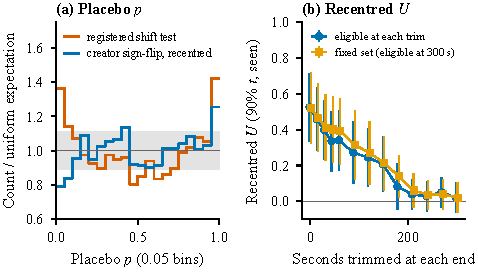
\includegraphics[width=\columnwidth]{floats/fig_hthree.pdf}
\caption{H3's calibration and trim. (a) Placebo: sets per $p$ bin over the count expected under a uniform $p$, with a
binomial 90\% band (CAL, sets of \HThreeCreators{} seen creators); the registered circular-shift $p$ piles up in both
tails because it holds creators fixed, while a creator sign-flip on the recentred $U$ stays near nominal. (b) Trim:
recentred $U$ (creator-equal mean, 90\% $t$ interval) against the seconds trimmed from each end, seen creators only.
Exploratory.}
\label{fig:hthree}
\end{figure}

\begin{figure}[t]
\centering
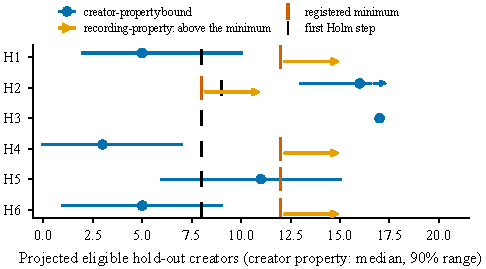
\includegraphics[width=\columnwidth]{floats/fig_eligibility.pdf}
\caption{Projected eligible hold-out creators per hypothesis, under CAL's two bounds: eligibility as a property of the
creator (filled dot, the bound the announcement of 02:50 rests on; median and 90\% range, a dashed arrow where the upper
end is not drawn) and of each recording (arrow from the minimum: its median lies above the minimum; neither its median
nor its range is drawn, as the projections are capped at a count this paper withholds). Solid tick, the registered ``not run'' minimum; black tick, the smallest count at which an exact sign-flip can
pass 0.005 (\MinCreatorsOneSided{} one-sided, \MinCreatorsTwoSided{} two-sided). H3 shows its realised count; H5 is one upper bound
from pilot titles. Projections from model-coded pilot labels, not counts.}
\label{fig:eligibility}
\end{figure}

\begin{figure*}[tp]
\centering
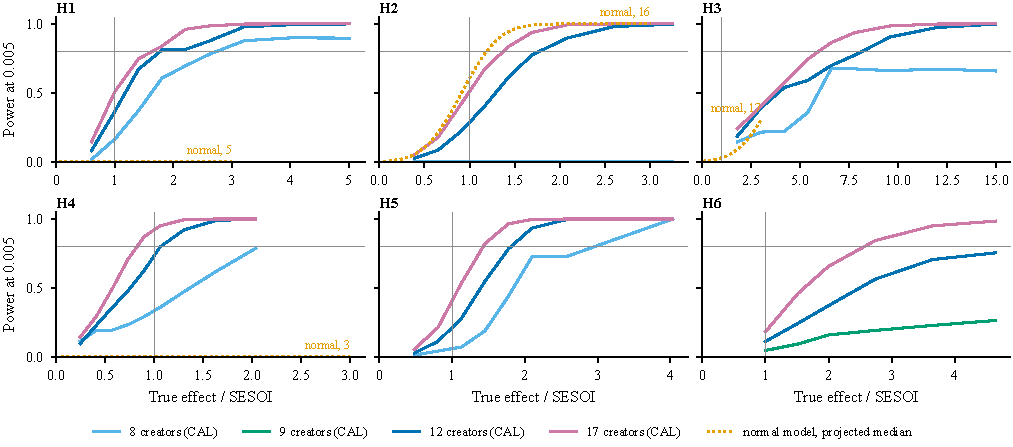
\includegraphics[width=\textwidth]{floats/fig_power.pdf}
\caption{Power of a creator sign-flip at the first Holm step (0.005) against the true effect in units of the smallest
effect of interest: CAL's seen-creator analogues (H1 to H5) and CAL's planted simulation for H6, at the creator counts
named in the legend, and, dotted, a normal model at the projected median for H1 to H4 only. Analogues carry no labels
and are not hypothesis quantities.}
\label{fig:power}
\end{figure*}

\begin{figure}[t]
\centering
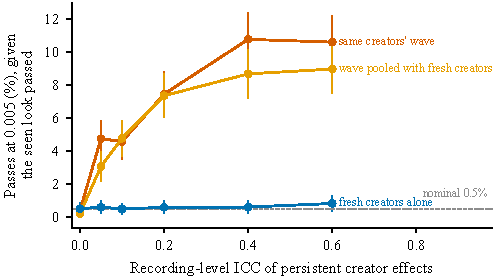
\includegraphics[width=\columnwidth]{floats/fig_plasmode.pdf}
\caption{Why a wave of the same creators cannot replicate. Plasmode under a population null with persistent creator
effects (seen cluster sizes and within-creator pace residuals): share of cases in which a one-sided test at 0.005 passes,
given that an exploratory seen look passed at 0.05. A wave of the same creators passes in
\PlasmodeWaveLo--\PlasmodeWaveHi\% of cases across the simulated recording-level ICCs; fresh creators alone pass at about
nominal. Bars: 90\% Monte Carlo intervals.}
\label{fig:plasmode}
\end{figure}

\paragraph{Deviations and contacts.} Table~\ref{tab:deviations} and Figure~\ref{fig:timeline} carry
Section~\ref{sec:deviations}; Table~\ref{tab:contacts} lists every hold-out contact named in Section~\ref{sec:limits}.
The \NCloudOnlyObjects{} cloud-only metadata objects are to be read once, after freeze 2, in one logged read-only pass
(registry 03:08; moved here from Section 9 by the page limit, results round); the registry records no such read yet.

% INTEGRATOR (2026-11-21): the deviation table is about three pages tall; the builder writes it in three parts of
% consecutive, numbered rows. The class column uses the seven classes of Section 8.
\begin{table*}[tp]
\centering
\small
% tab_deviations.tex: GENERATED by the private builder build_numbers.py at 2026-11-26T03:59:48Z; label tab:deviations. The writer adds the float,
% the caption and the label. Sources: a private file of the run (named in the private build record); REG/registry.md
% Part 1 of 6. Rows: D6 (to 00:50 UTC), the registry's deviation table (A10 Part 8, rows from 01:10 UTC), and registry rows written after it was last brought up to date.
{\tiny\setlength{\tabcolsep}{2pt}
\begin{tabular}{@{}rp{0.065\textwidth}p{0.1\textwidth}p{0.42\textwidth}p{0.09\textwidth}p{0.16\textwidth}l@{}}
\toprule
 & UTC & Applies to & As done (against the registry of 20 Nov, 19:47 UTC) & Known then & Direction & Class \\
\midrule
1 & found 2026-11-20 about 23:00 (panel round 2) & H3 reference distribution & shift reference ignores variation between creators; creator-level placebo rejects 1.3-1.6\% at nominal 0.5\% (CAL) & H3 hold-out and seen results & looser than R1 as registered & looser \\
2 & found after the test & H3 estimand centring & U has mean -0.063 under its own reference; recentred seen value 0.083 (F5) & yes & neutral (bias, not a choice) & neutral \\
3 & 20:38 (freeze) without the audit & H3 interval against CA & percentile creator-then-recording bootstrap; CA had not run before the hold-out was spent (F11) & no & looser & looser \\
4 & 20:38 & CA-1 coverage audit and planted-effect check & skipped for H3 & no & looser & looser \\
5 & 20:39 & Leave-one-creator-out range & not reported for H3 & no & looser & looser \\
6 & 2026-11-20 20:49 & H3 verdict and A6 & 'supported' reported, then H3 dropped by the owner (A6, 20:49 UTC) after reading the result & yes (H3 hold-out and seen results) & neutral (claim withdrawn, row kept) & neutral \\
7 & 2026-11-20 20:49 & H3 registered wave replication & closed by A6: not tested again as confirmatory & yes & neutral & neutral \\
8 & 2026-11-20 20:39-20:49 & A5 stricter verdict & 'supported' also needs the 90\% interval over creators to exclude 0, for hypotheses not yet run & yes (H3) & stricter & stricter \\
9 & 2026-11-20 19:47 (with the freeze) & A2 'uninformative' pruning & no operational definition of 'uninformative' written & no & looser (undefined) & looser \\
10 & 2026-11-20 about 22:45 & A8 no human check & no person checks any label; strongest verdict 'supported (model-coded)' & yes (H3, bridge, pilots) & looser & looser \\
11 & 2026-11-20 about 22:45 & A9 H8 dropped; stricter amendments in principle & H8 dropped, counted as run with p = 1; sign-flip p, fixed Holm count of 10, 'not determinable' outcome approved in principle & yes & H8: neutral; amendments: stricter & neutral \\
12 & 11-21 16:07 & A10 exact text of the stricter amendments & A10 and its companion parts 2 to 7 entered in the registry from A10-draft.md (its hash cited there), before freeze 2 and any hold-out label & SP, SP-C; no hold-out label & stricter & stricter \\
13 & 2026-11-20 about 22:50 & A11 verification by language models & a third, larger model and known-answer texts stand in for the human check & yes & looser than R7; neutral against A8 & looser \\
14 & 2026-11-20 about 23:10, after the H3 test & Selection rule of the cohort & 'channelling mediums' stated by the owner & yes & neutral (descriptive, post hoc) & neutral \\
15 & 2026-11-20 about 22:45 & Holm count & count fixed at 10, unrun at p = 1 (A9 in principle) & yes & stricter & stricter \\
16 & pending at 00:50; settled 11-21 16:06 & H7 and H9 smallest effects & H7 margin 0.01 shown to be unreachable; block-reference units proposed (F9); settled at 16:06 (row 87): H9 keeps the placeholder 0.2 standardised units (a mixed deviation), H7 is not run & seen creators only & to be set; must not be looser; settled 16:06 & other \\
17 & 2026-11-20 22:30 and 23:10 & Budget & 120 USD (caps 60/50/4, 115 total), then a warning with a 250 USD loop guard & yes & neutral for inference & neutral \\
18 & 2026-11-20 13:00 to 23:07 & Hold-out definition and contacts & four contacts before freeze 2 (snapshot tables, run report heat map at 20:09, H3 run, panel metadata load) plus the planned TABLE extraction; the contact table lists every contact, those of 21 November included (public-output generators, the one-off seen-derivative script) & partly & looser than the stated rule & looser \\
19 & 2026-11-21 about 00:30 & Freeze-1 instruments & checkability (time window 0.55, place not published (fewer than 5 creators)) and titles (not published: fewer than 5 creators) failed; middle model made the record with larger-model adjudication & pilot results on seen and check creators & looser (gate failed, instrument kept) & looser \\
20 & 11-21 commit 22:56:59 & - & Hold-out contact log added & PAN & disclosure & other \\
21 & 11-21 commit 23:03:43 & H1, H4, H6 & Primary definitions: broad own voice; an offer alone does not end a claimed voice & CAL, G (voice pilots) & neutral; chosen before any label of the frozen instrument & neutral \\
22 & 11-21 01:10 & reliability, wording, exploratory & V4 and V6 merged for reliability reporting; "guided steps" wording; the adjudicating model fixed; the other-vendor reader added; timeline built after the seen forecast labels & G (verification pilot) & neutral; the other-vendor reader is stricter & neutral \\
23 & 11-21 01:15 & H1, H4, H6 & Voice: variant B, with the one revision spent on gate C (0.834 against 0.90); if gate C fails again, H1, H4 and H6 are not run & G & stricter (consequence fixed beforehand) & stricter \\
24 & 11-21 01:15 & H6 & Ask check input states the number of candidates; ask gate rerun & G & neutral & neutral \\
25 & 11-21 01:15 & H1, H4, H6 & Middle model is the voice record on the hold-out; H4's yardstick comes from small-model labels on all seen recordings & G & neutral & neutral \\
26 & 11-21 01:15 & all labelled & Gate rule: combined rule; an instrument below its floor means "not run", p = 1 & G & stricter (A10.5) & stricter \\
27 & 11-21 01:15 & H2, H5 & Forecast protocol defaults: H5's share and minimum hits as CAL drafted them; H2 also on one-voice recordings; calendar class; titles without a cue coded as not presented; seen creators labelled first & CAL & H5's minimum guarded (A10.4); the rest neutral & guarded \\
28 & 11-21 01:20 & H6 & Ask check: context units are for reading only; a class listed twice is accepted & G & neutral & neutral \\
\bottomrule
\end{tabular}}

\caption{Deviations from the registry frozen \RegistryFrozenStamp{} (hypotheses SHA-256 prefix
\HypothesesShaPrefix), part 1 of 6: row number; UTC of the change; what it applies to; what was done against the
registry; results known at the time; direction as recorded; and its class (stricter; guarded by amendment A10; neutral;
looser; mixed: stricter for some uses and looser for others, or of a direction not known in advance, outside the guard;
exploratory; budget or operations; other: disclosure, correction of the record, the freeze-1 entry, reporting (the
public results file and its republications), or not yet decided).
\NDeviationRows{} rows: the paper review's table, the registry's deviation table (A10 Part 8, entered at \ATenStamp;
its rows of contacts, of the freeze-1 entry and of corrections of the record included), and the registry rows written
after that table was last brought up to date (16:06 to 23:34); no deviation is listed twice. The relayed-voice merge of
02:55 is classed looser here, against A10's own record, and applies to H1 and H6 (registry 04:55 (a)), where A10 lists
H1 and H4 (Section~\ref{sec:instruments}).}
\label{tab:deviations}
\end{table*}

\begin{table*}[tp]
\centering
\small
% tab_deviations_b.tex: GENERATED by WORK/build_numbers.py at 2026-11-22T00:15:32Z; label tab:deviations. The writer adds the float,
% the caption and the label. Sources: REV/build-descriptive/out/D6/D6-deviation-table.csv; REG/registry.md
% Part 2 of 6. Rows: D6 (to 00:50 UTC), the registry's deviation table (A10 Part 8, rows from 01:10 UTC), and registry rows written after it was last brought up to date.
{\tiny\setlength{\tabcolsep}{2pt}
\begin{tabular}{@{}rp{0.065\textwidth}p{0.1\textwidth}p{0.42\textwidth}p{0.09\textwidth}p{0.16\textwidth}l@{}}
\toprule
 & UTC & Applies to & As done (against the registry of 20 Nov, 19:47 UTC) & Known then & Direction & Class \\
\midrule
29 & 11-21 01:30 & H6 & Ask gate C failed (0.721), so the one revision is used: the union of two draws. The gate row is not switched to the row that passed. A second failure means H6 is not run (declared before the rerun). Output cap set & G & stricter or neutral & stricter \\
30 & 11-21 02:00 & - & Budget 130 USD with a hard stop; batch interface; restart in the guarded environment, with no label, gate or estimate changed & - & budget, operations & budget \\
31 & 11-21 02:20 & H6 & Ask rerun: gate C passes; gate B fails for the small check, so the middle model becomes the ask-check record & G & neutral (both measured on the same runs) & neutral \\
32 & 11-21 02:25 (note 3) & -; H6 rows & Discovery stopped by a hard cap; the H6 census keeps the middle-model find; a hold-out preparer for the rewording rows & - & budget; stricter (rows) & budget \\
33 & 11-21 02:40 & instruments & Known-answer battery cap raised for the six items that check frozen instruments & G & budget & budget \\
34 & 11-21 02:45 & all labelled & Listing repair (25 seen transcripts had no listing row); format of the freeze-2 record & - & neutral (data repair) & neutral \\
35 & 11-21 02:50 (note 4) & HR & Hold-out robustness rows released on `verification\_passed` and `verification\_basis`, not `human\_passed` & - & neutral (follows A8) & neutral \\
36 & 11-21 02:50 (note 4) & paper & The paper becomes a measurement-and-protocol paper; first-round results are reported as model-coded descriptions & REV & stricter (claims) & stricter \\
37 & 11-21 02:50 (note 4) & H1, H4, H6 & A8 stands; H1, H4 and H6 announced as probably not determinable (median 5, 3 and 5 eligible creators against 12) & REV, CAL & stricter (announced in advance) & stricter \\
38 & 11-21 02:50 (note 4) & measurement & Anchor against text made or edited by people: word error rate against text made or edited by people, on seen creators; grid-shift re-decode & REV, BR & exploratory & exploratory \\
39 & 11-21 02:50 (note 4) & public outputs & Public outputs: rows and bins with fewer than 5 creators merged; dashboard statements corrected & REV & disclosure & other \\
40 & 11-21 02:50 (note 4) & all & Registry additions before freeze 2: A10; hold-out-only primary; "uninformative" defined; exploratory reporting plan & REV, CAL & A10 guarded; "uninformative" stricter for the claims; hold-out-only primary has less power and, with the rule of 04:55 (h), cannot make a verdict easier to reach (Part 4) & guarded \\
41 & 11-21 02:50 (note 4) & H2, H5 & H2 and H5 revised at the analysis level (M9). H2: flagged statements, and reduced to its parts with at least 5\% prevalence. H5: excludes units next to a self-naming cue; three Q2 assignments. Second readings by another model & REV, G & changes registered estimands before any label; direction not known in advance; the rows without each change are reported beside (Part 7) & mixed \\
42 & 11-21 02:50 (note 4) & H3 & H3: the wave replication reported as not run; one logged rerun of the frozen H3 code on the hold-out after freeze 2 (exploratory) & REV, CAL & exploratory & exploratory \\
43 & 11-21 02:50 (note 4) & exploratory & Prediction timeline: methodological agnosticism; source types reported as separate rows & REV & exploratory; stricter wording & exploratory \\
44 & 11-21 02:50 (note 4) & - & Left to the owner: ethics, lawful basis, inclusion rule, external registration, unlinking the site & REV & not decided & other \\
45 & 11-21 02:53 & H2 (forecast class) & Forecast critic: one boundary sentence; forecast gates rerun; the known-answer relayed arm rescored & G (known-answer battery) & neutral (follows the codebook); before freeze 1 & neutral \\
46 & 11-21 02:53 & H1, H4, H6 & Voice: the middle model stays the hold-out record; seen voice descriptives come from the middle-model subset & G & neutral & neutral \\
47 & 11-21 02:55 & H1, H6 (H4: secondary row only; registry 04:55 (a)); A10 lists H1, H4 & Voice revision 3: relayed voice merged into claimed voice (Part 5) & G & looser (post-hoc merge decided after the gate result; by the letter of plan 3.4, not run; A10 records it as: stricter (consequence fixed in plan 3.4)) & looser \\
48 & 11-21 02:55 & H1, H4, H6 & Voice settings for freeze 1; the middle model at effort low, a recorded deviation from the plan's effort rule & G & neutral & neutral \\
49 & 11-21 commit 02:56:03 & record & Stamps of nine rows corrected from 03:00 to 02:50 & - & correction of the record & other \\
50 & 11-21 03:08 & all & Order of spending under the 130 USD stop & - & budget & budget \\
51 & 11-21 03:08 & freeze 1, HR, H1, H4, H6 & Replacement of the human check in every rule that names it (Part 2) & G, REV & follows A8; no floor lowered & neutral \\
52 & 11-21 03:08 & H1, H2, H4-H7, H9, H10 & A10 with its guard (Part 1) & CAL, REV & stricter or guarded & stricter \\
53 & 11-21 03:08 & all labelled tests & Recognizer rule (Part 6) & PAN & stricter & stricter \\
54 & 11-21 03:08 & exploratory; H3 wording & Panel decisions adopted: H3 wording; topic reading A, decided at about 02:30 UTC after its stage-1 results; and others & PAN, CAL & exploratory; one reading chosen after its results, stated openly & exploratory \\
55 & 11-21 03:12 & H2 (forecast class); timeline & Forecast critic: the relayed-forecast sentence counted as its one revision; gate D passes on its lower bound; the ten-class label fails stability (0.77 against 0.85) and is a description only; the known answer is not changed & G (gates, known-answer battery) & neutral for the registered uses, which need F1 against the rest (gate D's contrast) & neutral \\
\bottomrule
\end{tabular}}

\caption{Deviations from the registry, part 2 of 6 (columns as in part 1).}
\label{tab:deviations-b}
\end{table*}

\begin{table*}[tp]
\centering
\small
% tab_deviations_c.tex: GENERATED by WORK/build_numbers.py at 2026-11-22T01:51:42Z; label tab:deviations. The writer adds the float,
% the caption and the label. Sources: REV/build-descriptive/out/D6/D6-deviation-table.csv; REG/registry.md
% Part 3 of 6. Rows: D6 (to 00:50 UTC), the registry's deviation table (A10 Part 8, rows from 01:10 UTC), and registry rows written after it was last brought up to date.
{\tiny\setlength{\tabcolsep}{2pt}
\begin{tabular}{@{}rp{0.065\textwidth}p{0.1\textwidth}p{0.42\textwidth}p{0.09\textwidth}p{0.16\textwidth}l@{}}
\toprule
 & UTC & Applies to & As done (against the registry of 20 Nov, 19:47 UTC) & Known then & Direction & Class \\
\midrule
56 & 11-21 03:12 & H2 (forecast class); timeline & Class of record for every registered and timeline use: F1 against the rest, whose stability passes gate C (0.93). Gate C in the annotation plan reads "at least 85\% of units keep their class", the ten-class label; the coarser class was chosen at 03:12, after the ten-class row had failed & G (the failed ten-class row) & deviation from gate C's wording, chosen after its result and stated openly: looser for the gate (a two-class label keeps its value more easily than a ten-class one); neutral for the registered uses, which read only F1 against the rest & looser \\
57 & 11-21 03:12 & H2 (checkability) & Production adjudication of checkability keeps the large model fixed at 01:10; the recorded gate figures, made with another tier, stay as recorded and the difference is reported & G & neutral (decided before these figures) & neutral \\
58 & 11-21 03:18 & exploratory & Entrance experiment: pattern version 1 is primary, version 2 (revised after the check reading) a labelled secondary row; the names lexicon pinned to the store version of its seen run; counts as cue counts and upper bounds & G (check reading), PAN & exploratory; version 2 made after a reading, labelled & exploratory \\
59 & 11-21 03:21 & H1, H4, H6; HR & Other-vendor voice check (gate VG-6) fixed before its sealed figures are opened: comparator the stored OpenAI majority; on failure H1, H4 and H6 are flagged and capped at "not determined" and the HR (b, c) money returns; on a pass it serves the HR (b, c) release rule, overriding the programme's rule that the fallback cannot pass & G (figures sealed) & stricter for H1, H4 and H6; looser for the HR release (the fallback can pass), fixed before the figures & mixed \\
60 & 11-21 03:21 & instruments (H2, H5) & Verification before freeze 1: typed guided fields and shard sizes kept; the sentence-code instrument stays at one unit per call, the gated form, against the protocol text's 15 per call; the time instrument's role stability reported as a limit & G & neutral; a deviation from the protocol text, the gated form kept & neutral \\
61 & 11-21 04:55 & - & Budget guard at worst case: the 130 USD hard stop and every tag cap are tested with every open batch job at its worst case plus the new step's worst case; the protocol's one repeat reserves its full output cap; batch reservations hold twice the measured mean output (at most the cap), measured on seen pilot and gate stores; production waves under 128 USD at worst case; the verification shard's pins amended for four files after its requests were rebuilt and found unchanged & FRV & budget, operations; the hard stop holds at worst case again & budget \\
62 & 11-21 04:55 & H1, H2, H4-H7, H9, H10 & Decisions on the freeze-readiness open points: (a) H4's primary stays the embodied voice (V2) as registered, V2 + V3 a secondary row without a verdict (Part 5); (b) the model-stratified recognizer row built as written (Part 6); (c) H5's HKSJ random-effects row (A10.7); (d) each registered version under the guard uses the interval hypotheses.md registers for it (guard); (e) "a possibility" leaves H2's shared-wording flag (Part 7); (f) label files opened only after the permission check (Part 4); (g) "not determinable" when either guarded version is (guard); (h) no replication wave, the hold-out the only confirmation sample (Part 4); (i) H7's verdict against both margins (A10.6); (j) the wider Mantel-Haenszel interval until the coverage repeat (A10.4); (k) H6's registered version uncentred, its null mean reported (A10.7); (l) A10.k = CAL A(7 + k) in text and code; (m) H10 not run in the first round, its readers replaced before it is run (Part 2); (n) the simulation battery on the earlier code stopped, a new one on the final code & FRV, DBL, CAL & (a), (d) and (k) follow the registered text; (b) and (c) add rows; (g), (h), (i) and (j) stricter; (e) changes H2's primary sample, direction not known in advance, and removes a selection on the outcome; (f), (l), (m) and (n) neutral or operations & stricter \\
63 & 11-21 04:55 & H2, H5 & Second reading (02:50) recorded on seen check creators; the checkability codebook is not changed before freeze 1; H2 gets a sensitivity row in which a time window taken only from the period of the talk counts as NO; the reading covers checkability and the sentence codes, not commitment & DBL & stricter (one more row); the primary already does not count such a time window read as YES, so the row differs from it only where it is read "cannot tell" (Part 7) & stricter \\
64 & 11-21 freeze-1 entry: 04:58:22 & instruments & Freeze 1 of the instruments: record, configuration, models, code and 83 prompt and schema files fixed by hash; seen production unlocked, hold-out and other labels only after freeze 2 & G, FRV, DBL & procedure freeze & other \\
65 & 11-21 04:59 (note 5) & freeze 1; HR & Freeze 1 does not wait for the known-answer battery's last voice batches (pending since about 02:47 UTC), against the rule of 03:08 that freeze 1 waits on the battery's pre-set rules (Part 2); the request-id fixture retaken for the four forecast-critic lists only & G (the battery's finished items) & deviation from the 03:08 rule, stated with its reason: looser for freeze 1's timing; no instrument is affected (each has spent its revision), and the battery still serves the paper and the HR (b, c) release & looser \\
66 & 11-21 04:59 & H1, H4, H6; HR & Gate VG-6 opened after freeze 1 with its seal verified: kappa 0.91 (0.84 to 0.95) on claimed, own and other voice, 0.91 (0.83 to 0.96) on the embodied contrast; it passes, so no vendor flag applies to H1, H4 and H6, and VG-6 meets its part of the HR (b, c) release & VG & neutral (a result read under the meaning fixed at 03:21) & neutral \\
67 & 11-21 05:00 & seen labels & Seen-creator production starts through the batch interface under freeze 1, one driver per instrument, with its cost projection (about 20 USD) reported before sending and spending stops on three of its lines & G & budget, operations & budget \\
68 & 11-21 06:33 & seen labels; known-answer battery & The heads of the seen voice and forecast chains move to the standard interface after their batch jobs had returned nothing for 80 to 85 minutes (open jobs cancelled first; request ids and bodies unchanged; about 2 USD extra); three known-answer batch jobs re-sent after cancellation at 05:44 & - & budget, operations & budget \\
69 & 11-21 06:36 & exploratory outputs & Exploratory reporting plan and its addendum 1 registered by hash. Lead's decisions in the addendum: the public rows of the word-error-rate anchor keep machine texts of different origin apart and withhold the pooled automatic row, a departure from the plan's section 3; the diagnostic cards' verdicts are not reported; the missing measures of the grid-shift re-decode (BR-GS) are built from the existing re-decodes; the abstract gives the caption figure as agreement only; the anchor's hold-out part runs after freeze 2 as a logged contact & BR-b & exploratory; hashed after the anchor's first tables, which the addendum names; the departure is stated with its reason & exploratory \\
\bottomrule
\end{tabular}}

\caption{Deviations from the registry, part 3 of 6 (columns as in part 1).}
\label{tab:deviations-c}
\end{table*}

\begin{table*}[tp]
\centering
\small
% tab_deviations_d.tex: GENERATED by WORK/build_numbers.py at 2026-11-22T01:51:42Z; label tab:deviations. The writer adds the float,
% the caption and the label. Sources: REV/build-descriptive/out/D6/D6-deviation-table.csv; REG/registry.md
% Part 4 of 6. Rows: D6 (to 00:50 UTC), the registry's deviation table (A10 Part 8, rows from 01:10 UTC), and registry rows written after it was last brought up to date.
{\tiny\setlength{\tabcolsep}{2pt}
\begin{tabular}{@{}rp{0.065\textwidth}p{0.1\textwidth}p{0.42\textwidth}p{0.09\textwidth}p{0.16\textwidth}l@{}}
\toprule
 & UTC & Applies to & As done (against the registry of 20 Nov, 19:47 UTC) & Known then & Direction & Class \\
\midrule
70 & 11-21 06:39 & seen labels & Every small-model stage of the seen chain (sentence codes, asks find and small-model check) moves to the standard interface after its batch jobs were cancelled and collected; the middle-model and title stages stay in batch; extra cost of all moves about 5 USD; the committed spend projected after the seen and hold-out chains stays under the 120 USD warning only if the hold-out small-model stages go through batch or the queue clears & - & budget, operations & budget \\
71 & 11-21 contact log: about 03:00 to 06:35 & public outputs & Hold-out contact: the public-output generators loaded the run report's per-recording timing cache, hold-out and other creators included, to rebuild distribution tables; no word, label or hypothesis statistic was read or produced & - & disclosure; one generator no longer loads the cache and the other two are changed to read seen creators only for positional measures (closed by the entry of 06:49:10) & other \\
72 & 11-21 06:44 & H2, H5, H6, H9; freeze 2; paper & Decisions on the second verification of the hypothesis code, before freeze 2 and any hold-out label: (1) a seen-only permission path: before freeze 2 the analysis code may open labels/seen only, refusing any other path and any record whose group is not seen, for the freeze-2 constants, CAL part (f) and the A10.7 null-mean check; the path is part of the code freeze 2 hashes (Part 4; A10.7); (2) one freeze-2 record, `llm/freeze2.json` with the six keys of 02:45, which the analysis code checks against its modules (Part 4); (3) H6's amended OE and Mantel-Haenszel rate ratio centred per recording, the registered version as registered (A10.4; guard); (4) H9's creator-bootstrap interval drawn creators, then recordings (R1) in both versions, with fewer draws allowed in the simulation battery if stated (A10.7; guard); (5) A5 for H5 and H6 on both the t interval of the creator OE values and the wider Mantel-Haenszel interval (A10.1; A10.4); (6) H6's $\delta$ for "uninformative" stays log 2 (Part 3); (7) the M9 revisions stay outside the guard, the rows without them reported with their own verdicts (Part 7); (8) H2's FRAME row stays as built (Part 7); (9) creator-by-model strata for H5 in the model-stratified row (Part 6); (10) times cited in the paper are commit times (this table); (11) the full simulation battery started at 04:57 on earlier code was stopped at 06:42, a new one is to run on the final code & SV, FRV & (1) neutral for every verdict: a narrow exception to (f) that opens only seen labels, which freeze 1 released for production, and computes no hypothesis quantity; (2) neutral, fails closed; (3) guarded: it changes the amended statistic and removes a centring fault in H6's predicted direction; (4) and (6) follow the registered text (for (6), the stricter $\delta$ of log 1.5 was not taken); (5) stricter; (7) and (8) neutral, confirming Part 7; (9) a sensitivity row only, now exactly within one model; (10) record; (11) operations & neutral \\
73 & 11-21 contact log: 06:49:10 (note 6) & public outputs & Hold-out contact: a one-off script loaded the run report's per-recording timing cache once and kept only the rows of the 71 seen creators (by the creator sets of freeze 1), writing a seen-only derivative; nothing was computed on any other row, and the script refuses to run again. Since then no generator reads the cache: whole-run counts come from ledger fields, every timing measure from the seen derivative & - & disclosure; closes the generators' use of hold-out timing rows & other \\
74 & 11-21 07:50 (note 7) & seen labels & The forecast critic (about 42,600 small-model requests) was first sent through batch to save about 2.2 USD, under a rule fixed beforehand: cancel if under half is back after 30 minutes. None of the first 3,000 came back in 30 minutes, so its batch jobs were cancelled and collected and it runs through the standard interface (estimate 4.4 USD, run limit 6 USD). Seen titles, voice and asks are done & - & budget, operations; the rule fixed beforehand was applied & budget \\
75 & 11-21 commit 08:24:06 (note 7) & record & The row of 07:50 moved from the hold-out contact log into the table of decisions (commit message: "insertion slip"); its text unchanged & - & correction of the record & other \\
76 & 11-21 08:33 & known-answer battery; HR & Known-answer battery: its voice parts (the revision-3 arms and the voice audit), waiting in the small model's batch queue since about 02:47 (cancelled and re-sent once at 05:44), finish through the standard interface after both lanes' open batch jobs were cancelled and collected; a few hundred requests, about 1 USD, inside the battery's tag cap tested at worst case & - & budget, operations & budget \\
77 & 11-21 09:10 & HR; paper & Known-answer battery complete (constructed texts; exploratory, an upper bound and not accuracy on the corpus): with voice revision 3 the small model's recovery rose on the relayed-voice, own-offer and interview arms, and the canary gates pass for voice, asks and forecasts. With VG-6 (04:59), the row states both parts of the HR (b, c) release rule met; HR (b, c), a tier-5 line, starts only within the 120 USD rule of 03:08 & G (the battery's results) & neutral: a result read under rules fixed before it (03:08, 03:21); no instrument changes & neutral \\
78 & 11-21 09:19 (note 8) & H5, H6; freeze 2 & Decisions on the third verification of the hypothesis code, before freeze 2 and any hold-out label: (1) H6's amended version keeps OE centred per recording, but its reference becomes a conditional Monte Carlo draw under the per-recording null (each recording's asks from a binomial with its claimed share, given its ask count) in place of the sign-flip, because exact enumeration showed the one-sided sign-flip rejecting 1.93\% at 0.005 with one ask a creator at a claimed share of 0.3; the battery gains a null scenario with shares below one half and 1 to 3 asks a creator (A10.4); (2) the A10.7 null-mean tolerance of the OE versions is a tenth of the smallest effect on the OE scale, not 0.1 on the share scale (A10.7); (3) the null check keeps recordings without an ask file, as the analysis does (A10.7); (4) a verifier's test file that globbed the production label tree leaves the code's package; (5) the hypothesis code is committed to the analysis branch before freeze 2, and A10 keeps its `**A10.` heading for the labelling side's check (Part 4); (6) H5's stratified-row choice for a stratum without hits on one side stays as written (weight at most 0.25), stated as a limit & V3 & (1) guarded (the amended version only); the row said it "can only make a verdict harder to reach", which the row of 11:08 corrects; replaced at 11:08 (1); (2) stricter (a tighter check); (3) neutral: the check reads the creators the analysis reads; (4) neutral: protects the hold-out; (5) record; (6) a sensitivity row, a stated limit & guarded \\
79 & 11-21 11:08 & H6 & Correction to the row of 09:19: the conditional reference does not "only make a verdict harder to reach"; on some data its p is below the sign-flip's & V4 & correction of the record & other \\
\bottomrule
\end{tabular}}

\caption{Deviations from the registry, part 4 of 6 (columns as in part 1).}
\label{tab:deviations-d}
\end{table*}

\begin{table*}[tp]
\centering
\small
% tab_deviations_e.tex: GENERATED by WORK/build_numbers.py at 2026-11-22T01:51:42Z; label tab:deviations. The writer adds the float,
% the caption and the label. Sources: REV/build-descriptive/out/D6/D6-deviation-table.csv; REG/registry.md
% Part 5 of 6. Rows: D6 (to 00:50 UTC), the registry's deviation table (A10 Part 8, rows from 01:10 UTC), and registry rows written after it was last brought up to date.
{\tiny\setlength{\tabcolsep}{2pt}
\begin{tabular}{@{}rp{0.065\textwidth}p{0.1\textwidth}p{0.42\textwidth}p{0.09\textwidth}p{0.16\textwidth}l@{}}
\toprule
 & UTC & Applies to & As done (against the registry of 20 Nov, 19:47 UTC) & Known then & Direction & Class \\
\midrule
80 & 11-21 11:08 & H6, H9; freeze 2 & Decisions on the fourth verification, before freeze 2 and any hold-out label: (1) H6's amended reference redraws asks by cluster (asks in the same checked unit range or in adjacent units form one cluster; each cluster's voice drawn with the recording's claimed share), and the p that enters the guard is the larger of this cluster-level conditional p and the sign-flip p of OE, so that neither the sparse low-share case (where the sign-flip over-rejects) nor bursts of asks in one voice (where an ask-level reference over-rejects: 7.7\% at 0.005 for bursts of 3) can carry a verdict alone; 99,999 draws in the analysis; a burst scenario in the battery; H6's detectable-effect note from the battery (A10.1; A10.4; guard); (2) H9's content words exclude every variant of the frozen family table as well as the NAMES v2 list forms; (3) contractions whose parts are function words count as function words; (4) masking NAMES v2 forms everywhere (the flat-list form of the released mask) stays, stated as a choice, and the 9 seen transcripts without a stated model enter the model-stratified row as unknown model (Part 6); the seen feature files are written again with (2) and (3) before the freeze-2 constants are computed & V4, FT & (1) stricter than the sign-flip of OE that A10.4 drafted, since the amended p is never below it; against the reference of 09:19 the direction depends on the data; inside the guard; (2) construct, both versions of H9: removes a mechanical raise of same-family content similarity, in H9's predicted direction; (3) construct, both versions of H9, direction not known in advance; (4) a stated choice and a sensitivity row; the re-written feature files: operations & stricter \\
81 & 11-21 11:10 & seen labels; freeze 2 & Seen-creator production complete under freeze 1 (05:01 to 11:10): voice, asks, sentence codes and forecasts for all 1,293 English recordings of the 71 seen creators, titles for the 71 creators; production measured 24.27 USD, committed spend 111.89 USD against the 120 USD warning and the 130 USD hard stop; no hold-out or other-group recording was labelled; the freeze-2 constants are computed from these labels alone & - & budget, operations & budget \\
82 & 11-21 12:52 & H6 & Correction to the row of 11:08: with 99,999 draws the p is reproducible (seeded by its label), but inside about 0.0045 to 0.0055 the side of 0.005 still depends on the draws & V5 & correction of the record & other \\
83 & 11-21 12:52 & H6, H9; freeze 2 & Decisions on the fifth verification, before freeze 2 and any hold-out label: (1) H6's clusters: asks within 5 units of each other (about one minute of speech) form one cluster, chaining; a 10-unit window is a sensitivity row; H6's result states that dependence of asks beyond the window is not modelled; the battery gains a scenario with asks one to three units apart at shares below one half (A10.4; guard); (2) the analysis counts asks of one class whose unit ranges overlap once (the union of two find draws can return one ask twice); the instrument is frozen and unchanged (A10.4; guard); (3) H9's contraction rule also splits ain't and y'all into function words; (4) the analysis refuses a bundle whose feature files mix feature versions (Part 4); (5) the wide mask of 11:08 (2) stays (every token of every family variant, about 6\% of content tokens), which can only lower same-family content similarity; (6) the freeze-2 constants are computed from the seen labels through the seen-only path after these changes, recomputed by a second reader and entered in `constants.py` (Part 4) & V5, FT, SP & (1) corrects a level fault of 11:08's clusters (a burst of 3 asks 2 units apart at s = 0.3, 17 creators: 1.93\% at 0.005 with the clusters of 11:08, 0.23\% with the 5-unit window; A10.4); the amended p stays at least the sign-flip p, so stricter than A10.4's draft; inside the guard; its limit beyond the window is stated; (2) a counting correction in both versions of H6, direction not known in advance; (3) construct, both versions of H9 (20 tokens on the seen transcripts); (4) stricter: fails closed; (5) confirms 11:08 (2); (6) procedure: the constants come from seen labels alone, after every change above (14:00 UTC) & stricter \\
84 & 11-21 13:05 & exploratory outputs & Exploratory reporting plan, addendum 2 registered by hash (`c35f316b...`): it corrects addendum 1 (normaliser version 2 made at 03:31:13 to 03:31:26 UTC; the edit of 03:43 changed only the trimming rule), records version 1 as rebuilt exactly and run (rates not printed by the pair rule), the public inventory form, the precision check without a band, the choices of the grid-shift re-decode made while building, the per-cell interval seeds, the merged rows, and the dominance and pair rules applied to every public cell of the anchor and the re-decode; and it fixes the hold-out anchor's reading of caption makers before freeze 2 & BR-b & exploratory; corrects the record of addendum 1 (row of 06:36); every choice made after a result is named & exploratory \\
85 & 11-21 15:14 & H1, H4, H5, H9; freeze 1; freeze 2 & Before freeze 2. (1) Freeze 1, amendment 1: the hold-out and other-group feature files that H1, H4, H5 and H9 read had no guarded path (hold-out transcripts open only while produce.py is the program, and produce.py had no feature step), as the analysis code's README foresaw. produce.py gains a command `features GROUP` that runs only after freeze 2 for a group other than seen, loads the analysis package's `features.py` only at the SHA-256 that freeze 2 pins for it (so seen and hold-out features come from one source), uses the seen run's names and families inputs (hashes pinned in freeze 2) and writes `labels/GROUP/features` with the same feature version; no instrument, prompt, model, setting or request changes. Freeze 1 is written again for the changed produce.py; the record of 04:58:22 UTC is kept beside it, and seen labels keep their freeze time (Part 4) & SP, DV & operations: a new freeze-1 entry that adds a guarded path for the hold-out features, computed by the code and with the inputs of the seen run; no instrument, label or verdict rule changes & guarded \\
86 & 11-21 15:14 & H4, H5, H6; HR; A10 text & (2) Settled for the A10 text, before freeze 2: the ask merge of 12:52 (2) is a counting correction in both versions of H6, outside the guard (Part 1; A10.4; guard); with CAL part (f) not run, the simulation battery on synthetic creators stands in for planted-effect recovery and the Mantel-Haenszel interval stays the wider of two (A10.4; A10.7 point 3); a recording whose model is in dispute stays out of the model-stratified row (Part 6); H4's yardstick keeps its minimum of 40 own-voice forms per creator, set in code before any seen label existed (0.1474 over 52 creators; 0.156 over 60 without it), stated as a choice (Part 4); H6's registered half-count version stays uncentred under the guard (seen null mean -0.137; A10.7 point 3; guard); the HR (b, c) release also needs CAL's two eligibility conditions, read after the hold-out labels, and its money rule (Part 2); the full battery runs on the frozen code after freeze 2 and fills H6's detectable-effect note (A10.2) & SP, SP-C, V5, DV & the ask merge: a classification of the text, the counting of 12:52 (2) unchanged; the battery for recovery: a weaker check than the seen-label check the draft of A10.7 asked for, read by no verdict; the wider interval: as 04:55 (j), stricter; disputed recordings: a sensitivity row only; H4's yardstick: a stated choice made after both values were known on seen labels, keeping the rule the code held before them; the yardstick scales H4's standardised drops, so it moves the conditions that compare a drop with 0.5 (the kept value is the smaller) and not the sign-flip p, direction not fixed; H6's registered version: follows the registered text (04:55 (k)); the HR (b, c) release: follows the rule of 03:08 and A10.2, stricter than the row of 09:10 read alone; the battery after freeze 2: operations, and H6's detectable-effect note is filled after freeze 2 rather than before it as A10.2 asks of the others & stricter \\
\bottomrule
\end{tabular}}

\caption{Deviations from the registry, part 5 of 6 (columns as in part 1).}
\label{tab:deviations-e}
\end{table*}

\begin{table*}[tp]
\centering
\small
% tab_deviations_f.tex: GENERATED by WORK/build_numbers.py at 2026-11-22T00:15:32Z; label tab:deviations. The writer adds the float,
% the caption and the label. Sources: REV/build-descriptive/out/D6/D6-deviation-table.csv; REG/registry.md
% Part 6 of 6. Rows: D6 (to 00:50 UTC), the registry's deviation table (A10 Part 8, rows from 01:10 UTC), and registry rows written after it was last brought up to date.
{\tiny\setlength{\tabcolsep}{2pt}
\begin{tabular}{@{}rp{0.065\textwidth}p{0.1\textwidth}p{0.42\textwidth}p{0.09\textwidth}p{0.16\textwidth}l@{}}
\toprule
 & UTC & Applies to & As done (against the registry of 20 Nov, 19:47 UTC) & Known then & Direction & Class \\
\midrule
87 & 11-21 16:06 & H9; freeze 2 & last points before freeze 2: (1) H9's smallest effect of interest stays at the registry's placeholder, 0.2 standardised units, adopted as the value, since no rule for setting it from seen creators was registered and choosing one with the seen cells computed would let seen data pick the threshold; the seen creators' H9 contrast is a description only; (2) CAL part (f) did not run: every detectable-effect note comes from the full simulation battery on the frozen code, read by no verdict; (3) the hypothesis package normalised to LF line endings, the seen feature files reproduced byte for byte; (4) freeze 1 written again for produce.py with the feature step & SP, SP-C; no hold-out label & mixed (a deviation from the wording 'set from the seen creators', of a direction not known in advance, outside the guard); (2) to (4) neutral or operations & mixed \\
88 & 11-21 16:13 & labels & hold-out production starts under both freezes (16:11), through the standard interface (the small model's batch queue returned nothing to a probe), with run limits and its cost projected before sending; R-hold drawn from ledger fields only & SP-C; no hold-out label & budget, operations & budget \\
89 & 11-21 16:26 & HR; hold-out labels & the hard stop, tested at worst case, refused a standard-interface chunk of the hold-out voice labels (16:20), so the middle model's voice labels went through batch; the money left goes to the registered chain first; HR part (a) and HR (b, c) not bought & hold-out labels in production or done; no test result & budget (HR (a) and HR (b, c), registered robustness rows, not bought) & budget \\
90 & 11-21 16:48 & labels & hold-out production complete under both freezes (16:11 to 16:47), feature files by the frozen feature step; committed spend past the owner's warning of 120 USD, under the hard stop & hold-out labels in production or done; no test result & budget, operations & budget \\
91 & 11-21 17:29 & R-hold; HR & the reliability driver's plan mode refused R-hold (placeholder answers changed the stitched maps and so the request ids); its fix kept as a patch, not applied, so that both freezes stay as written; R-hold runs in run mode with per-command run limits; the HR rewording arms are not run (not released) & hold-out labels in production or done; no test result & budget, operations (no rule of the reliability design changes; only the plan mode's cost preview is lost) & budget \\
92 & 11-21 18:17 & R-hold; HR & R-hold's middle-model arms move from batch to the standard interface after the first batch, its open job cancelled and collected first; HR part (a) not bought, as it would leave less than 1 USD under the hard stop at worst case & hold-out labels in production or done; no test result & budget, operations (HR (a) not bought) & budget \\
93 & 11-21 18:41 & first-round labels; HR & all first-round labelling complete (hold-out, the checkability check on the hold-out, R-hold, the other group); 126.70 USD committed (125.93 measured, the rest held by unreleased reservations of ended runs), past the warning and under the hard stop; no further model call planned for the first round & hold-out labels in production or done; no test result & budget (HR (a) and HR (b, c) not bought) & budget \\
94 & 11-21 19:30 & first-round test inputs; gates & decisions on the first-round test inputs: (1) a driver outside the freeze ran the frozen reliability report body for R-hold, whose frozen command stops in the HR block, and its figures were accepted; (2) voice gate A read per instrument, as the plan states it, a per-stage reading would fail it; (3) the owner's 00:30 exception applied to the title codes as recorded, not extended; (4) the second-model row of H4 reported with the flag 'labels below the reliability floor'; (5) the public results print each failed gate with its figure & R-hold gates; the results for (4) & mixed: (2) and (3) are choices made after a gate result was computed and before the results were read; (1) operations (the frozen code computed every figure); (4) adds a flag after the results and claims nothing & mixed \\
95 & 11-21 20:48 & public results & public results file written: eligible counts stated against their minimums, each failed gate with its figure, figures resting on fewer than 5 creators withheld & first-round results & reporting (no verdict changes) & other \\
96 & 11-21 21:52 & simulation battery & full simulation battery complete on the frozen code, resumed from its checkpoint with fewer workers after a memory stop & first-round results & budget, operations (read by no verdict) & budget \\
97 & 11-21 22:33 & public results & public results file republished at 21:50 (converter fixes; every hold-out checkability part withheld under the engineer's stricter test) and at 22:33 under one rule for every agreement figure, decided by the lead: the positive code comes from 5 or more creators in each reading, and the creators with a statement the readings code differently are 0 or 5 or more; a minor code both readings give alike is not a cell of its own. Under it the hold-out place and quantity parts and the R-hold asks stability figure C are withheld, and three hold-out checkability parts withheld at 21:50 (time window, named actor, observable outcome) are published & first-round results & reporting (no verdict changes; a rule chosen when the figures it would publish were known, for one standard with the guard of the R-hold figures) & other \\
98 & 11-21 23:17 & exploratory outputs (status L, F2) & exploratory round of the reporting plan started under the owner's delegation: the outputs that need no model call, each run, verified and fixed; outputs that need model calls reported as not run; every hold-out run a logged contact & first-round results; no output of this round read & exploratory (code written after freeze 2, a deviation from the plan's 'code frozen in the freeze-2 record', declared before any of these outputs is read) & exploratory \\
99 & 11-21 23:34 & public results & public results file republished at 23:33 after the final pre-push check: the R-hold asks relative-recall figure E withheld under the 22:33 rule (the accepted asks one finder missed come from fewer than 5 creators), as figure C was; counts of valid calls and quotations in the gate texts given as shares without their shortfalls; the file's small-cells statement states the 22:33 rule & first-round results & reporting (no verdict changes) & other \\
\bottomrule
\end{tabular}}

\caption{Deviations from the registry, part 6 of 6 (columns as in part 1).}
\label{tab:deviations-f}
\end{table*}

% INTEGRATOR (2026-11-21): floats/fig_timeline.pdf was re-drawn by the builder with the events after 01:10 UTC; the
% numbers on the marks are keyed in floats/tab_timeline_key.tex, set below the figure.
\begin{figure*}[tp]
\centering
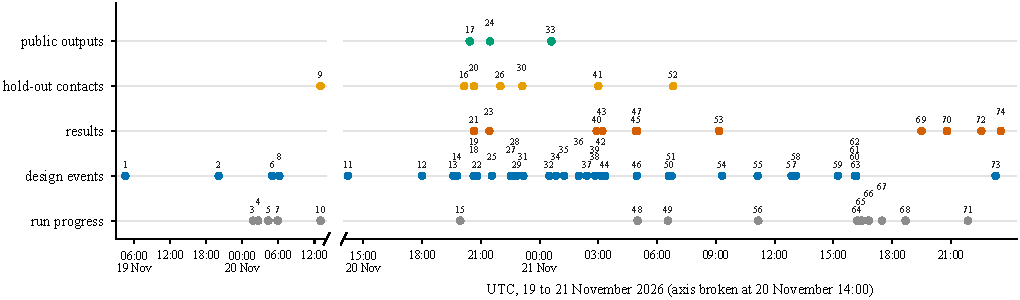
\includegraphics[width=\textwidth]{floats/fig_timeline.pdf}

\medskip
% tab_timeline_key.tex: GENERATED by WORK/build_numbers.py at 2026-11-22T00:15:32Z; label fig:timeline (key). The writer adds the float,
% the caption and the label. Sources: REV/build-descriptive/out/D6/D6-timeline-events.csv; REG/registry.md; LLM/freeze.json
% Key to the numbers of fig_timeline, in two halves side by side.
{\tiny\setlength{\tabcolsep}{2pt}
\begin{tabular}{@{}rllp{0.3\textwidth}rllp{0.3\textwidth}@{}}
\toprule
 & UTC & Lane & Event &  & UTC & Lane & Event \\
\midrule
1 & 19 Nov 04:31 & design & roster table lists 74 channels & 38 & 21 Nov 02:50 & design & paper becomes measurement and protocol \\
2 & 19 Nov 20:03 & design & roster of 101 channels first committed & 39 & 21 Nov 02:50 & design & H1, H4, H6 announced not determinable \\
3 & 20 Nov 01:45 & run & downloads paused (1,946 of 1,976 archived) & 40 & 21 Nov 02:55 & results & voice revision 3 gates \\
4 & 20 Nov 02:38 & run & transcription starts (first progress row) & 41 & 21 Nov 03:00 & contacts & public-output generators load the per-recording timing cache (to about 06:35) \\
5 & 20 Nov 04:19 & run & language fallback phase & 42 & 21 Nov 03:08 & design & content of amendment A10 and its guard written (entered at freeze 2 at the latest) \\
6 & 20 Nov 04:57 & design & owner closes the download goal (30 final failures) & 43 & 21 Nov 03:12 & results & forecast critic revision \\
7 & 20 Nov 05:52 & run & English-first ordering starts (ledger line 251) & 44 & 21 Nov 03:21 & design & VG-6 meaning fixed before opening \\
8 & 20 Nov 06:08 & design & English-first and creator-language rules committed & 45 & 21 Nov 04:55 & results & second reading recorded \\
9 & 20 Nov 13:00 & contacts & first panel tables include 32 hold-out files & 46 & 21 Nov 04:58 & design & freeze 1 \\
10 & 20 Nov 13:00 & run & snapshot of 1,213 finished transcripts (paper numbers) & 47 & 21 Nov 04:59 & results & VG-6 opened: passes \\
11 & 20 Nov 14:13 & design & experiment catalogue (28 experiments) committed & 48 & 21 Nov 05:00 & run & seen production starts \\
12 & 20 Nov 18:00 & design & paper draft committed & 49 & 21 Nov 06:33 & run & seen chains: heads move to the standard interface \\
13 & 20 Nov 19:36 & design & ten candidate hypotheses proposed & 50 & 21 Nov 06:36 & design & reporting plan and addendum 1 registered by hash \\
14 & 20 Nov 19:47 & design & registry frozen (hypotheses.md hash) & 51 & 21 Nov 06:44 & design & hypothesis code: second verification (H6 OE centred per recording) \\
15 & 20 Nov 19:57 & run & run closes: 1,699 of 1,731 recordings transcribed & 52 & 21 Nov 06:49 & contacts & one-off script cuts that cache to the seen creators \\
16 & 20 Nov 20:09 & contacts & run report with position heat map of every creator & 53 & 21 Nov 09:09 & results & known-answer battery complete (voice revision 3) \\
17 & 20 Nov 20:26 & outputs & findings dashboard first published & 54 & 21 Nov 09:19 & design & hypothesis code: third verification (H6 conditional reference) \\
18 & 20 Nov 20:38 & design & H3 procedure frozen & 55 & 21 Nov 11:08 & design & hypothesis code: fourth verification (H6 cluster reference; H9 content words) \\
19 & 20 Nov 20:39 & design & A5 stricter verdict added (after the H3 result) & 56 & 21 Nov 11:09 & run & seen production complete \\
20 & 20 Nov 20:39 & contacts & H3 run opens every English hold-out transcript & 57 & 21 Nov 12:52 & design & hypothesis code: fifth verification (H6 clusters within 5 units; asks counted once) \\
21 & 20 Nov 20:39 & results & H3 result: passes registered rule, interval includes 0 & 58 & 21 Nov 13:05 & design & reporting plan addendum 2 registered by hash \\
22 & 20 Nov 20:49 & design & A6: H3 dropped by the owner & 59 & 21 Nov 15:14 & design & freeze-1 amendment (feature step) decided; A10 text settled \\
23 & 20 Nov 21:26 & results & bridge result: word measures agree, timing differs & 60 & 21 Nov 16:06 & design & H9's smallest effect: the registry's placeholder adopted (a deviation) \\
24 & 20 Nov 21:28 & outputs & dashboard results tab (H3 'supported by the registered rule') & 61 & 21 Nov 16:06 & design & freeze 1 written again (amendment 1, feature step) \\
25 & 20 Nov 21:34 & design & A7: second-round panel gets control and budget & 62 & 21 Nov 16:07 & design & amendment A10 entered \\
26 & 20 Nov 22:00 & contacts & panel coverage script loads \textasciitilde{}415 hold-out metadata files & 63 & 21 Nov 16:10 & design & freeze 2 \\
27 & 20 Nov 22:32 & design & A3 change: budget 120 USD & 64 & 21 Nov 16:13 & run & hold-out production starts (16:11); R-hold drawn \\
28 & 20 Nov 22:45 & design & A8 no human check; A9 H8 dropped & 65 & 21 Nov 16:26 & run & hard stop refuses a standard chunk at worst case (16:20) \\
29 & 20 Nov 22:50 & design & A11 verification by language models & 66 & 21 Nov 16:48 & run & hold-out production complete (16:47) \\
30 & 20 Nov 23:07 & contacts & TABLE whitelisted metadata extraction (planned; done once) & 67 & 21 Nov 17:29 & run & R-hold in run mode (plan mode refused, 16:33) \\
31 & 20 Nov 23:10 & design & selection rule stated; budget becomes a warning & 68 & 21 Nov 18:41 & run & all first-round labelling complete; HR (a), HR (b, c) not bought \\
32 & 21 Nov 00:30 & design & freeze-1 decisions: two instruments failed gates & 69 & 21 Nov 19:30 & results & first-round tests run (18:54 to 19:03); decisions on their inputs \\
33 & 21 Nov 00:36 & outputs & public outputs reduced to distributions & 70 & 21 Nov 20:48 & results & public results file first written \\
34 & 21 Nov 00:50 & design & lead decides under the owner's delegation & 71 & 21 Nov 21:52 & run & full simulation battery complete \\
35 & 21 Nov 01:15 & design & voice: one revision spent & 72 & 21 Nov 22:33 & results & results republished under one rule for agreement figures \\
36 & 21 Nov 02:00 & design & budget 130 USD hard stop & 73 & 21 Nov 23:17 & design & exploratory round of the reporting plan started \\
37 & 21 Nov 02:25 & design & channeler discovery closed & 74 & 21 Nov 23:33 & results & first-round results published (current version) \\
\bottomrule
\end{tabular}}

\caption{Design timeline in UTC, one lane each for run progress, design events, results, hold-out contacts and public
outputs; the key below the plot names each numbered event. Times are commit times or the time stated in the cited
record. A selection of events to the registry's latest row (\TimelineEndStamp): first-round labelling (to
\LabellingDoneStamp), the tests and the decisions on their inputs, the full simulation battery, the first-round results
and their republications (the current version last) and the start of the exploratory round; the contacts of 21
November included; the deviations themselves are in Table~\ref{tab:deviations}.}
\label{fig:timeline}
\end{figure*}

\begin{table*}[tp]
\centering
\small
% tab_contacts.tex: GENERATED by the private builder build_numbers.py at 2026-11-26T03:59:48Z; label tab:contacts. The writer adds the float,
% the caption and the label. Sources: REG/registry.md; REG/hypotheses.md; a private file of the run (named in the private build record)
% Part 1 of 7. Counts of recordings, durations, dates and languages from the run ledger are not contacts. None of these contacts produced a statistic about a registered hypothesis on hold-out text other than H3's registered test (registry).
{\scriptsize\setlength{\tabcolsep}{2pt}
\begin{tabular}{@{}p{0.13\linewidth}p{0.22\linewidth}p{0.44\linewidth}p{0.18\linewidth}@{}}
\toprule
When (UTC) & What touched the hold-out & What was read or written & Status \\
\midrule
20 Nov, about 13:00 (during the run) & The snapshot tables of the first analyst panel (catalogue section 2) & 32 audio files of hold-out creators entered recording-level descriptive tables before the hold-out was declared & Known since the catalogue; stated in the paper's limitations \\
20 Nov, before 19:47 & the first panel's position pilot (H3 disclosure) & drew on 83 creators, more than the 71 seen, so early files of some hold-out creators probably entered it; it produced per-position first-person rates, the reading that suggested H3 & stated in the paper's limitations \\
20 Nov, 20:09 (D6) & The run report and the findings dashboard: speech by position in the recording, recordings by length and share without speech & Timing measures (no words) of every transcribed recording, hold-out creators included, shown in a position heat map and per-creator tables & Found by the second-round panel; stated in the paper's limitations. Fixed 2026-11-21: the run report, the paper figures and the dashboards now draw positional displays from seen creators only, and publish distributions instead of per-creator rows (owner's decision on public identifiers) \\
20 Nov, 20:39 & The registered test of H3, as its frozen procedure allowed & Every English hold-out transcript was opened by the frozen code; the code opened each file more than once across its count-only and full runs & Allowed by the H3 freeze; listed for completeness \\
20 Nov, about 21:50 to 22:15 & A coverage script of the second-round panel (social scientist, round 1) & About 415 metadata files of hold-out recordings were loaded in full (title, description, tags among their fields) and the presence of fields was counted for non-seen creators. The panel reports that no hold-out text was analysed or written out & Breach of the round's rule, found by two other panel members; no hold-out text field is to be extracted before freeze 2 \\
20 Nov, 23:07:10 to 23:07:35 & The TABLE item of the second-round programme & 1,778 local metadata files opened once (hold-out 437, other 57); only time stamps and durations written for non-seen recordings & planned contact, disclosed in advance; done once \\
21 Nov, about 03:00 to 06:35 & The public-output generators of the privacy work (run\_report.py, publish\_progress.py --rebuild, dashboard\_data.py) & They loaded the run report's per-recording cache, which holds timing measures by position (coverage by tenth, quiet stretches, speech seconds) of every transcribed recording, hold-out and other creators included, to rebuild distribution tables with 5 or more creators per cell; no word, label or hypothesis statistic was read or produced & Found by the privacy verifier; dashboard\_data.py no longer loads it; the other two generators are changed to read seen creators only for positional measures \\
21 Nov, at the paper review's build of rv-R3 (before the exploratory reporting plan was written at about 03:00 UTC; exact time not recorded) & Exploratory round, Paper review build (rv-R3): rv-R3's Bland-Altman bins and percentiles & The registered per-recording bridge table, which holds one other-group creator's recording. Displayed or written: recording-level values entered the build's private tables; nothing of them is published & Contact (other group); logged late under D6 (D42). Contact flag: none; the parts that rest on it stay held (D42) \\
21 Nov, 06:49:10 & The one-off script seen\_derivative.py of the privacy work & It loaded the run report's per-recording cache once and kept only the rows of the 71 seen creators (by the creator sets of freeze 1), writing a seen-only derivative; nothing was computed on any other row, and the script refuses to run again. Since then no generator reads the cache: whole-run counts come from ledger fields, every timing measure from the seen derivative & Logged; closes the generators' use of hold-out timing rows \\
21 Nov, about 18:40 to 18:50 & A driver outside the freeze that ran the frozen reliability report body for R-hold (frozen 'reliability report rhold' stops on the relative-recall arm in the HR block) & It read the R-hold reliability arms' label files (hold-out creators) and wrote the report's aggregate figures to a private folder; the frozen code computed every figure; nothing else was read or produced & Logged; the figures are accepted as R-hold's report (decision row of this time) \\
21 Nov, 18:54 to 19:03 & The registered first-round tests (run.py analyse under both freezes) & The frozen code read the hold-out label and feature files and wrote the private report & Allowed by the freezes; listed for completeness \\
\bottomrule
\end{tabular}}

\caption{Every contact with hold-out recordings outside a procedure frozen for it: UTC, what touched the hold-out, what
was read or written, status. Counts of recordings, durations, dates and languages from the run ledger are not contacts.
The registry records that no contact produced a statistic about a registered hypothesis on hold-out text other than
the registered tests run by their frozen procedures (H3; then H1, H2, H4, H5, H6 and H9).}
\label{tab:contacts}
\end{table*}

\paragraph{Exploratory outputs.} The reporting plan lists every exploratory output with its place;
Table~\ref{tab:outputs} counts them by status. The seen-creator model-coded descriptions made under freeze 1 are
pending: voice \PendLabV, asks \PendLabA, forecasts \PendLabF, sentence codes \PendLabS, titles \PendLabT, recording
kinds \PendLabK.

\begin{table}[t]
\centering
\small
% tab_outputs.tex: GENERATED by the private builder build_numbers.py at 2026-11-26T03:59:48Z; label tab:outputs. The writer adds the float,
% the caption and the label. Sources: REG/exploratory-reporting-plan.md; REG/exploratory-reporting-plan-addendum-1.md; a private file of the run (named in the private build record)
% 114 outputs listed in the plan's section 6 tables (first code of each row); the status at report time from the round's status table (exploratory release). The full status table is in the exploratory release.
{\scriptsize\setlength{\tabcolsep}{3pt}
\begin{tabular}{@{}lp{0.72\linewidth}r@{}}
\toprule
Code & Status or place (plan section 6) & Outputs \\
\midrule
B & built on seen creators: reported in full & 51 \\
L & waits for first-round labels & 43 \\
F2 & waits for freeze 2 & 9 \\
X & will not run; reported with its reason & 4 \\
R & runs now without labels & 4 \\
N & waits for a decision or data & 2 \\
I & other & 1 \\
\midrule
S & supplement & 85 \\
M & main text & 29 \\
\midrule
\multicolumn{3}{@{}p{0.97\linewidth}}{\emph{Status at report time (plan section 9): the status table of the exploratory release, 172 outputs}} \\
 & reported in full, in the public-safe form of plan section 3 & 111 \\
 & not run; reported with its reason & 60 \\
 & superseded by a later output & 1 \\
\bottomrule
\end{tabular}}

\caption{Exploratory outputs of the reporting plan (SHA-256 prefix \PlanShaPrefix) and its addendum 1, counted by
status (reported; not run, with reason; pending; superseded) and by place (main text; appendix or supplement;
dashboard). The full status table, one row per output with its UTC time of run and code hash, is an online supplement.}
\label{tab:outputs}
\end{table}

\paragraph{External processing.} Table~\ref{tab:external} lists every service that received project data (ethics
statement).

% INTEGRATOR: moved here from the ethics statement by the P7 move log (build of 2026-11-21 07:05 UTC); caption as
% written by writer A. Third review round: full width (the column float ran over the page).
\begin{table*}[tp]
\centering
\small
% tab_external.tex: GENERATED by the private builder build_numbers.py at 2026-11-26T03:59:48Z; label tab:external. The writer adds the float,
% the caption and the label. Sources: a private file of the run (named in the private build record)
% Ledger read at 03:59 UTC (D8 rule rerun on counts only). Words = 0.75 x uncached input tokens, an estimate; each word was sent several times across instruments and runs.
{\scriptsize\setlength{\tabcolsep}{1.5pt}
\begin{tabular}{@{}p{0.21\linewidth}rrrp{0.12\linewidth}p{0.15\linewidth}@{}}
\toprule
Service: data category & Requests & Tokens (M) & Words (M, est.) & Third-party share & Retention, deletion \\
\midrule
\textbf{OpenAI API}: seen transcript windows (pilots, gates, checks) & 42{,}881 & 114.9 & 29.39 & 14.1\% [4.5, 24.1] (pilot) & vendor logs up to 30 days; store=false sent \\
\textbf{OpenAI API}: seen transcript windows (production) & 225{,}346 & 302.6 & 46.05 & 14.1\% [4.5, 24.1] (pilot) & as above \\
\textbf{OpenAI API}: hold-out transcript windows (production, after freeze 2) & 35{,}815 & 73.7 & 12.15 & 14.1\% [4.5, 24.1] (pilot) & as above \\
\textbf{OpenAI API}: hold-out transcript windows (reliability runs on R-hold, after freeze 2) & 13{,}420 & 32.2 & 4.18 & 14.1\% [4.5, 24.1] (pilot) & as above \\
\textbf{OpenAI API}: other-group transcript windows (production, after freeze 2) & 2{,}649 & 5.5 & 0.87 & 14.1\% [4.5, 24.1] (pilot) & as above \\
\textbf{OpenAI API}: seen transcript statements, with web search & 17{,}662 & 27.4 & 3.23 & -- & as above \\
\textbf{OpenAI API}: name forms from seen transcripts & 294 & 1.4 & 0.75 & -- & as above \\
\textbf{OpenAI API}: page text of seen recordings & 13{,}234 & 23.6 & -- & -- & as above \\
\textbf{OpenAI API}: constructed known-answer texts & 18{,}772 & 60.7 & -- & -- & as above \\
\textbf{OpenAI API}: public channel metadata, web search (discovery) & 26{,}338 & 89.4 & -- & -- & as above \\
\textbf{OpenAI API}: tests (no corpus data) & 192 & 0.1 & -- & -- & as above \\
\textbf{OpenAI API}: untagged requests (no tag recorded) & 5 & 0.0 & -- & -- & as above \\
\textbf{OpenAI Files and Batch}: request files & 116 jobs & -- & -- & -- & kept until deleted; deleted for 115 of 116 jobs \\
\textbf{Anthropic agents}: seen transcript windows (panels, review, cross-vendor reader) & not logged & -- & not logged & as in the pilot & terms not read \\
\textbf{Cloud drive}: audio and provenance records, all creators & -- & -- & -- & clients and audience in the audio & terms not read; owner holds \\
\bottomrule
\end{tabular}}

\caption{External processing of project data, from one read of the request ledger at \ExtStamp: \ExtRequests{} requests to the language-model API and \ExtInputTokensM{} million input tokens, which the rows sum to, and about \ExtWordsM{} million words of transcript-derived text with repeats (an estimate; words are not logged; transcript text from seen creators, and after freeze 2 from hold-out and other-group creators for the frozen instruments). The other rows carry constructed texts, public metadata of candidate channels or tests. Third-party share: model-coded voice-map pilot, 95\% creator bootstrap. Retention as each vendor documents it; the Anthropic terms were not read. This inventory is not an ethics determination.}
\label{tab:external}
\end{table*}
